% Options for packages loaded elsewhere
\PassOptionsToPackage{unicode}{hyperref}
\PassOptionsToPackage{hyphens}{url}
%
\documentclass[
]{article}
\usepackage{amsmath,amssymb}
\usepackage{lmodern}
\usepackage{iftex}
\ifPDFTeX
  \usepackage[T1]{fontenc}
  \usepackage[utf8]{inputenc}
  \usepackage{textcomp} % provide euro and other symbols
\else % if luatex or xetex
  \usepackage{unicode-math}
  \defaultfontfeatures{Scale=MatchLowercase}
  \defaultfontfeatures[\rmfamily]{Ligatures=TeX,Scale=1}
\fi
% Use upquote if available, for straight quotes in verbatim environments
\IfFileExists{upquote.sty}{\usepackage{upquote}}{}
\IfFileExists{microtype.sty}{% use microtype if available
  \usepackage[]{microtype}
  \UseMicrotypeSet[protrusion]{basicmath} % disable protrusion for tt fonts
}{}
\makeatletter
\@ifundefined{KOMAClassName}{% if non-KOMA class
  \IfFileExists{parskip.sty}{%
    \usepackage{parskip}
  }{% else
    \setlength{\parindent}{0pt}
    \setlength{\parskip}{6pt plus 2pt minus 1pt}}
}{% if KOMA class
  \KOMAoptions{parskip=half}}
\makeatother
\usepackage{xcolor}
\IfFileExists{xurl.sty}{\usepackage{xurl}}{} % add URL line breaks if available
\IfFileExists{bookmark.sty}{\usepackage{bookmark}}{\usepackage{hyperref}}
\hypersetup{
  pdftitle={Inferring true changes in microbial abundance from taxonomically-biased microbiome measurements},
  pdfauthor={Michael R. McLaren; Jacob T. Nearing; Amy D. Willis; Karen G. Lloyd; Benjamin J. Callahan},
  hidelinks,
  pdfcreator={LaTeX via pandoc}}
\urlstyle{same} % disable monospaced font for URLs
\usepackage[top=1in,bottom=1in,left=1.5in,right=1.5in]{geometry}
\usepackage{longtable,booktabs,array}
\usepackage{calc} % for calculating minipage widths
% Correct order of tables after \paragraph or \subparagraph
\usepackage{etoolbox}
\makeatletter
\patchcmd\longtable{\par}{\if@noskipsec\mbox{}\fi\par}{}{}
\makeatother
% Allow footnotes in longtable head/foot
\IfFileExists{footnotehyper.sty}{\usepackage{footnotehyper}}{\usepackage{footnote}}
\makesavenoteenv{longtable}
\usepackage{graphicx}
\makeatletter
\def\maxwidth{\ifdim\Gin@nat@width>\linewidth\linewidth\else\Gin@nat@width\fi}
\def\maxheight{\ifdim\Gin@nat@height>\textheight\textheight\else\Gin@nat@height\fi}
\makeatother
% Scale images if necessary, so that they will not overflow the page
% margins by default, and it is still possible to overwrite the defaults
% using explicit options in \includegraphics[width, height, ...]{}
\setkeys{Gin}{width=\maxwidth,height=\maxheight,keepaspectratio}
% Set default figure placement to htbp
\makeatletter
\def\fps@figure{htbp}
\makeatother
\setlength{\emergencystretch}{3em} % prevent overfull lines
\providecommand{\tightlist}{%
  \setlength{\itemsep}{0pt}\setlength{\parskip}{0pt}}
\setcounter{secnumdepth}{5}
\newlength{\cslhangindent}
\setlength{\cslhangindent}{1.5em}
\newlength{\csllabelwidth}
\setlength{\csllabelwidth}{3em}
\newlength{\cslentryspacingunit} % times entry-spacing
\setlength{\cslentryspacingunit}{\parskip}
\newenvironment{CSLReferences}[2] % #1 hanging-ident, #2 entry spacing
 {% don't indent paragraphs
  \setlength{\parindent}{0pt}
  % turn on hanging indent if param 1 is 1
  \ifodd #1
  \let\oldpar\par
  \def\par{\hangindent=\cslhangindent\oldpar}
  \fi
  % set entry spacing
  \setlength{\parskip}{#2\cslentryspacingunit}
 }%
 {}
\usepackage{calc}
\newcommand{\CSLBlock}[1]{#1\hfill\break}
\newcommand{\CSLLeftMargin}[1]{\parbox[t]{\csllabelwidth}{#1}}
\newcommand{\CSLRightInline}[1]{\parbox[t]{\linewidth - \csllabelwidth}{#1}\break}
\newcommand{\CSLIndent}[1]{\hspace{\cslhangindent}#1}
\usepackage{cancel}

% Define note environment based on example from https://bookdown.org/yihui/rmarkdown-cookbook/custom-blocks.html
\usepackage{color}
\usepackage{framed}
\setlength{\fboxsep}{.8em}
\newenvironment{rmdnote}{
  \definecolor{shadecolor}{RGB}{248,248,248}
  \begin{shaded}}
 {\end{shaded}}
\ifLuaTeX
  \usepackage{selnolig}  % disable illegal ligatures
\fi

\title{Inferring true changes in microbial abundance from taxonomically-biased microbiome measurements}
\author{Michael R. McLaren\footnote{North Carolina State University; send correspondence to \href{mailto:m.mclaren42@gmail.com}{\nolinkurl{m.mclaren42@gmail.com}}} \and Jacob T. Nearing\footnote{Dalhousie University} \and Amy D. Willis\footnote{University of Washington} \and Karen G. Lloyd\footnote{University of Tennessee} \and Benjamin J. Callahan\footnote{North Carolina State University}}
\date{2021-11-29}

\begin{document}
\maketitle

{
\setcounter{tocdepth}{2}
\tableofcontents
}
\hypertarget{preface}{%
\section*{Preface}\label{preface}}
\addcontentsline{toc}{section}{Preface}

\begin{verbatim}
#> working directory clean
\end{verbatim}

\emph{This manuscript was rendered from commit 8f81dd5293e7ef5bc3621bbbec2f5d7a41b6560d.}

\leavevmode\vadjust pre{\hypertarget{preface-warning}{}}%
\textbf{This in-progress manuscript is not intended for general scientific use.}
It is incomplete, has not been carefully reviewed, and may contain mistakes or other inaccuracies.
Please post comments or questions on the \href{https://github.com/mikemc/differential-abundance-theory/issues}{GitHub Issues page} or \href{m.mclaren42@gmail.com}{email Mike}.

This manuscript addresses the effect that the taxonomic bias inherent in microbiome measurement has on microbial differential-abundance analysis.
We describe the basic problem posed by taxonomic bias for measuring changes in the abundance of particular taxa across conditions and describe new strategies for mitigating the errors it induces.
Analyses of both relative and absolute abundances are considered.
In its current form, the manuscript sits somewhere between a standard scientific article and a monograph;
it consists of an article followed by a series of appendices which together give a comprehensive treatment of the implications of the McLaren, Willis, and Callahan (\protect\hyperlink{ref-mclaren2019cons}{2019}) model of taxonomic bias for differential-abundance analysis and experimental design.
It is licensed under a \href{https://creativecommons.org/licenses/by/4.0/}{CC BY 4.0 License}.
See \href{https://doi.org/10.5281/zenodo.4552717}{the Zenodo record} for how to cite the latest version.

\hypertarget{introduction}{%
\section{Introduction}\label{introduction}}

One of the most basic questions we can ask about microbial communities is: How do different microbial taxa vary in abundance---across space, time, and host or environmental conditions?
Marker-gene and shotgun metagenomic sequencing (jointly, MGS) can be used to measure the abundances of thousands of species simultaneously, making it possible to ask this question on a community-wide scale.
In these \emph{differential-abundance (DA) analyses}, the change in abundance of a microbial taxon across samples or conditions is used to infer ecological dynamics or find microbes that are associated with specific host diseases or environmental conditions.
Although standard MGS measurements lose information about total microbial density---and so are typically used to analyze the abundances of taxa relative to each other---new methods are increasingly used to provide absolute information, making it possible to analyze changes in absolute cell density.
In its various forms, DA analysis remain one of, if not the most, common forms of analyses applied to MGS data to elucide the inner workings of microbiomes and their relationships to host and environmental health.

Yet these DA analysis are built on a fundamentally flawed foundation.
MGS measurements are \emph{taxonomically biased}: Microbial species vary dramatically (e.g.~10-1000X) in how efficiently they are measured---that is, converted from cells into taxonomically classified sequencing reads---by a given MGS protocol (McLaren, Willis, and Callahan (\protect\hyperlink{ref-mclaren2019cons}{2019})).
This bias arises from variation in how species respond to each step in an MGS protocol, from sample collection to bioinformatic classification.
Although often associated with features specific to marker-gene sequencing---the variation among species in marker copy numbers and in primer-binding and amplification efficiencies---the existence of large variation in DNA extraction efficiencies and in the ability to correctly classify reads make taxonomic bias a universal feature of both marker-gene and shotgun measurements.
As a result of taxonomic bias, MGS measurements provide inaccurate representations of actual community composition and tend to differ across protocols, studies, and even experimental batches (Yeh et al. (\protect\hyperlink{ref-yeh2018taxo}{2018}),McLaren, Willis, and Callahan (\protect\hyperlink{ref-mclaren2019cons}{2019})).
These errors have been found in some cases to supersede sizable biological differences (e.g. Lozupone et al. (\protect\hyperlink{ref-lozupone2013meta}{2013})) and have may have contributed to failed replications of prominent findings in the human microbiome literature, such as the associations of Bacteroides and Firmicutes in stool with obesity (Finucane et al. (\protect\hyperlink{ref-finucane2014atax}{2014})) and the associations of certain species in the vagina of pregnant women with preterm birth (Callahan et al. (\protect\hyperlink{ref-callahan2017repl}{2017})).

The extent to which taxonomic bias has impacted the DA results in the scientific literature is unknown.
The typical approach taken to counter taxonomic bias is to standardize the measurement protocol used within a given study, with the (often tacit) assumption being that samples measured by the same protocol will be affected by bias in the same way and so the measured differences between samples will be unaffected.
For example, if taxonomic bias were to cause the measured proportion of a species to consistently be 10X too high, we would still be able to accurately infer the fold change in its proportion across samples (Kevorkian et al. (\protect\hyperlink{ref-kevorkian2018esti}{2018}),Lloyd et al. (\protect\hyperlink{ref-lloyd2020evid}{2020})).
Unfortunately, mathematical arguments and analysis of experiments with artificially constructed (`mock') communities demonstrate that this assumption is not always warranted:
Consistent taxonomic bias can lead to variable fold errors in species' proportions (Figure \ref{fig:basic-problem}, McLaren, Willis, and Callahan (\protect\hyperlink{ref-mclaren2019cons}{2019})).
These varying errors can lead to spurious conclusions for how the proportion of a taxon varies across samples, even in the direction of change (for example, causing a taxon that decreases appear to increase) (McLaren, Willis, and Callahan (\protect\hyperlink{ref-mclaren2019cons}{2019})).
Yet McLaren, Willis, and Callahan (\protect\hyperlink{ref-mclaren2019cons}{2019}) also found that certain types of DA analysis---those based on fold changes in the ratios among species---where robust to bias.
The implications of these findings for DA analysis of absolute abundances and for the joint analysis of variation of many species across many samples, as typically done in microbiome association testing, have yet to be investigated.

Here we use a combination of theoretical analysis, simulation, and re-analysis of published experiments to consider when and why taxonomic bias in MGS measurements leads to spurious results in DA analysis of relative and absolute abundance.
Our analysis clarifies how the folk wisdom that taxonomic bias does not affect the analysis of change across samples is only partially correct and can give a false sense of security in the accuracy of DA results.
Yet we also present several potential solutions---methods for quantifying, correcting, or otherwise accounting for the effect of taxonomic bias in DA analyses that can be deployed today with only modest changes to existing experimental and analytical workflows.
Over time, application of these methods to past and future experiments will provide crucial quantitative information about the conditions under which taxonomic bias creates spurious results for various DA methodologies.
Collectively, these methods and insights may provide practical solutions to taxonomic bias in DA analysis and the confidence that is necessary to codify the statistical findings of microbiome studies into readily-translatable scientific knowledge.

\begin{figure}
\centering
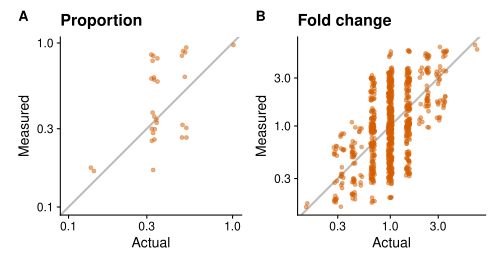
\includegraphics{figures/export-pdf/notebook/_posts/2021-10-27-illustrate-the-problem/illustrate-the-problem_files/figure-html5/brooks_lcrisp_prop_and_fc-1.pdf}
\caption{\label{fig:basic-problem}\textbf{Mock community experiments show that taxonomic bias can distort the measured fold change in an individual species' proportion across samples.} The figure shows the measured vs.~actual proportions for a single bacterial species, \emph{Lactobacillus crispatus}, in a set of bacterial cellular mock communities, and the resulting fold changes between community samples. The inconsistent error in the measured proportions of individual samples (Panel A) leads to inaccurate measurements of fold changes (Panel B). Mock communities were constructed and measured with 16S sequencing by Brooks et al. (\protect\hyperlink{ref-brooks2015thet}{2015}). The data was re-analyzed by McLaren, Willis, and Callahan (\protect\hyperlink{ref-mclaren2019cons}{2019}), who showed that despite the inconsistency of the errors in Panel A, taxonomic bias acted consistently across samples.}
\end{figure}



\hypertarget{abundance-measurement}{%
\section{How taxonomic bias affects abundance measurements}\label{abundance-measurement}}

To understand how bias affects the measured differential abundance between samples, we first consider how it affects measurements of individual samples.

\hypertarget{model-of-mgs-measurement}{%
\subsection{Model of MGS measurement}\label{model-of-mgs-measurement}}

Our primary tool for understanding the impact of taxonomic bias on MGS measurement is the theoretical model of MGS measurement developed and empirically validated by McLaren, Willis, and Callahan (\protect\hyperlink{ref-mclaren2019cons}{2019}).
This model is the simplest model of MGS measurement that includes multiplicative taxonomic bias while respecting the \emph{compositional} nature of sequencing measurements, in which the total read count for a sample is unrelated to its total cell number or density (Gloor et al. (\protect\hyperlink{ref-gloor2017micr}{2017})).
We consider a set of microbial species that are measured by a specific MGS protocol that extracts, sequences, and bioinformatically analyzes samples to assign reads to various microbial species.
We assume that assigned reads have been correctly assigned to the given species and sample.
Thus we ignore the possibility of contamination or false-positive taxonomic assignment, though we allow that many reads may not receive a taxonomic assignment and so ultimately be discarded.
Unless otherwise stated, we treat the sequencing measurement as deterministic, ignoring the `noise' or random error due to the random sampling of sequencing reads and other aspects of the MGS process.

Our model stipulates that the assigned read count of species \(i\) in sample \(a\) equals its cell density multiplied by a species-specific factor and a sample-specific factor,
\begin{align}
  \label{eq:measurement-model}
  \text{reads}_{i}(a)
  = \text{density}_{i}(a) \quad \cdot
    \underbrace{\text{efficiency}_{i}}_{\substack{\text{species specific,} \\  \text{sample independent}}}
    \cdot \quad
    \underbrace{\text{sequencing effort}(a)}_{\substack{\text{species independent,} \\  \text{sample specific}}}.
\end{align}
The species-specific factor is the \emph{relative measurement efficiency} (or \emph{efficiency} for short) of the species, which represents how much more easily that species is measured (converted from cells to assigned reads) relative to an abitrarily chosen reference species (McLaren, Willis, and Callahan (\protect\hyperlink{ref-mclaren2019cons}{2019})).
The sample-specific factor, which we call the \emph{sequencing effort} of the sample, reflects the fact that the number of reads per unit cell density varies among samples even in the absence of taxonomic bias due to variation in total density, library normalization, and total sequencing-run output.
Equation \eqref{eq:measurement-model} implies that the total reads from all species in the sample equal
\begin{align}
  \label{eq:total-reads}
  \text{total reads}(a)
    = \text{total density}(a) \cdot \text{mean efficiency}(a) \cdot \text{sequencing effort}(a),
\end{align}
where
\begin{align}
  \label{eq:mean-efficiency}
  \text{mean efficiency}(a) 
  \equiv \frac{\sum_{j}\text{density}_j(a)\cdot \text{efficiency}_j}{\text{total density}(a)}
\end{align}
is the average or mean efficiency of cells in the sample.

\hypertarget{relative-abundances-proportions-and-ratios}{%
\subsection{Relative abundances (proportions and ratios)}\label{relative-abundances-proportions-and-ratios}}

We distinguish between two types of species-level \emph{relative abundances}.
The first type consists of the \emph{ratios} among the abundances of two or more species, such as a ratio of 5:4:2 among three species.
The second type consists of the \emph{proportion} of an individual species, equal to its abundance divided by that of a particular root taxon (e.g.~Prokaryotes).
DA analyses of proportions consider how the proportion of a species changes indepently of other species, whereas DA analyses of ratios consider the conserted change in relative abundance among two or more species.
Although proportion-based analysis is dominant, microbiome researchers increasingly use ratio-based analyses adapted from the statistical framework of Compositional Data Analysis (CoDA).
The different manner in which taxonomic bias affects ratios vs.~proportions (McLaren, Willis, and Callahan (\protect\hyperlink{ref-mclaren2019cons}{2019})) forms the basis in subsequent sections for understanding the extent to which its effects cancel in DA analysis.

The standard measurement of the proportion of species \(i\) in sample \(a\) is given by the ratio of its read count to the total,
\begin{align}
  \label{eq:prop-meas}
  \widehat{\text{prop}}_{i}(a) = \frac{\text{reads}_i(a)}{\text{total reads}(a)}.
\end{align}
From Equations \eqref{eq:measurement-model}, \eqref{eq:total-reads}, and \eqref{eq:prop-meas}, it follows that
\begin{align}
  \label{eq:prop-error}
  \widehat{\text{prop}}_{i}(a)
  &= \text{prop}_{i}(a) \cdot \frac{\text{efficiency}_{i}}{\text{mean efficiency}(a)},
\end{align}
where \(\text{prop}_{i}(a) = \text{density}_{i}(a) / \text{total density}(a)\) is the actual proportion.
Equation \eqref{eq:prop-error} says that taxonomic bias creates a multiplicative error equal to the ratio of the species' efficiency to the mean efficiency in the sample.
Consequently, the same species can be over- or under-measured depending on the composition of the given sample (Figure \ref{fig:error-proportions}).
For instance, in samples from two hypothetical communities in Figure \ref{fig:error-proportions}, Species 3 has an efficiency of 6 and is under-measured in Sample 1 (which has a mean efficiency of 8.33) but over-measured in Sample 2 (which has a mean efficiency of 3.15).

The measured ratio between species \(i\) and \(j\) is given by the ratio of their read counts,
\begin{align}
  \label{eq:ratio-meas}
  \widehat{\text{ratio}}_{i/j}(a) = \frac{\text{reads}_i(a)}{\text{reads}_j(a)}.
\end{align}
From Equations \eqref{eq:measurement-model} and \eqref{eq:ratio-meas}, it follows that
\begin{align}
  \label{eq:ratio-error}
  \widehat{\text{ratio}}_{i/j}(a)
%  \frac{\text{reads}_{i}(a)}{\text{reads}_{j}(a)}
  &= \frac{\text{density}_{i}(a)}{\text{density}_{j}(a)} \cdot \frac{\text{efficiency}_{i}}{\text{efficiency}_{j}}.
\end{align}
The fold error in the ratio between two species simply equals the ratio in their efficiencies and is therefore constant across samples.
For instance, in the example of Figure \ref{fig:error-proportions}, the ratio of Species 3 (with an efficiency of 6) to Species 1 (with an efficiency of 1) is over-estimated by a factor of 6 in both communities despite their varying compositions.

\begin{figure}
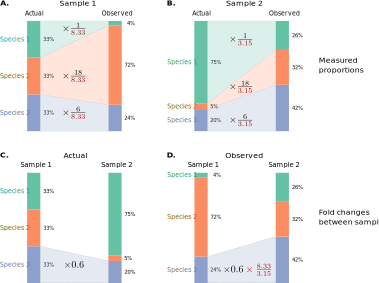
\includegraphics[width=0.9\linewidth]{figures/export-pdf/figures/illustrations/error-proportions} \caption{\textbf{Taxonomic bias creates sample-dependent multiplicative errors in species proportions, which can lead to inaccurate fold changes between samples.} Top row: Error in proportions measured by MGS in two microbiome samples that contain different relative abundances of three species. Bottom row: Error in the measured fold-change in the third species that is derived from these measurements.}\label{fig:error-proportions}
\end{figure}



\textbf{Difference between species proportions and species ratios:}
Consistent taxonomic bias at the species level creates a consistent fold error in the ratios among species, but a varying fold error in the proportions of individual species.
But a proportion is, after all, just a ratio between two taxa in which the denominator taxon is the entire taxonomic domain under study.
The difference in behavior from that of ratios between species arises because the efficiency of higher-level taxa, which consist of the aggregate of many species, varies across samples with the changing relative abundances among its constituent species.

\hypertarget{absolute-abundances-cell-densities}{%
\subsection{Absolute abundances (cell densities)}\label{absolute-abundances-cell-densities}}

A wide range of experimental methods exist for converting the relative-abundance information in MGS measurements into measurements of (absolute) cell densities;
however, these methods can be generally partitioned into two types, based on whether the absolute-abundance information derives from knowing the density of the total community or knowing the density of one or more individual species.

\textbf{Methods using the density of the total community:}
The total microbial density of a community can be assayed by a variety of methods (reviewed in Appendix \ref{review-absolute-methods}).
Once the total density is known, the density of individual species can be estimated by multiplying the total density by the species' proportions (as measured by MGS),
\begin{align}
  \label{eq:density-prop-meas}
  \widehat{\text{density}}_{i}(a) 
  &= \widehat{\text{prop}}_{i}(a) \cdot \widehat{\text{total density}}(a)
\\&= \text{reads}_{i}(a) \cdot \frac{\widehat{\text{total density}}(a)}{\text{total reads}(a)}.
\end{align}
We can rewrite the species' density measurements to account for the effect of taxonomic bias on the MGS proportions (Equation \eqref{eq:prop-error}) and any error in the total density measurement,
\begin{align}
  \label{eq:density-prop-error}
  \widehat{\text{density}}_{i}(a) 
  = \text{density}_{i}(a) \cdot \frac{\text{efficiency}_{i}}{\text{mean efficiency}(a)} 
%  \cdot \frac{\widehat{\text{total density}}(a)}{\text{total density}(a)}.
  \cdot \begin{array}{c} \text{fold error in} \\ \widehat{\text{total density}}(a) \end{array}.
\end{align}
The variable fold error that bias creates in the measured proportions directly transfers to the density measurements.

Taxonomic bias can also create systematic error in the total-density measurements (Appendix \ref{total-density-bias}).
For now, we suppose that the total density can be measured accurately;
later, Section \ref{solutions} describes how experiments might be designed such that taxonomic bias in the total density measurement offsets that in the MGS proportions, leading to a (more) consistent fold error in the measured densities.

\textbf{Methods using the density of one or more reference species:}
The density of one or more species can be directly measured using targeted measurement methods like species-specific qPCR; alternatively, the densities of one or more species may be thought to be constant across samples either from background knowledge or because they have been spiked in at a fixed density (these situations are reviewed in Appendix \ref{review-absolute-methods}).
These \emph{reference species} with known or constant density can be used to convert read counts to densities for all species.
For instance, given the density of a reference species \(r\), we can estimate the density of a focal species \(i\) by
\begin{align}
  \label{eq:density-ratio-meas}
%  \widehat{\text{density}}_{i}(a) = \frac{\text{reads}_{i}(a)}{\text{reads}_{r}(a)} \cdot \widehat{\text{density}}_{r}(a).
  \widehat{\text{density}}_{i}(a) = \text{reads}_{i}(a) \cdot \frac{\widehat{\text{density}}_{r}(a)}{\text{reads}_{r}(a)}.
\end{align}
Alternatively, if we only know that the reference species is constant, we can set \(\widehat{\text{density}}_{r}(a)\) in Equation \eqref{eq:density-ratio-meas} equal to 1 to estimate the density in unknown but fixed units, which is sufficient for multiplicative DA analysis.
(Appendix \ref{model-details} considers possible extensions to multiple reference species.)
It follows from Equation \eqref{eq:ratio-error} that the error caused by taxonomic bias in this density measurement is
\begin{align}
  \label{eq:density-ratio-error}
  \widehat{\text{density}}_{i}(a) 
  = \text{density}_{i}(a) \cdot \frac{\text{efficiency}_{i}}{\text{efficiency}_{r}} 
  \cdot \begin{array}{c} \text{fold error in} \\ \widehat{\text{density}_r}(a) \end{array}.
\end{align}
Here, it is the constant error in the measured ratio of species \(i\) to \(r\) that propagates into the density measurement.
There will generally be systematic error in the density of the reference species; however, if the systematic fold error is constant across samples, so will be that of the densities of other species.

\textbf{Differences between the two approaches:}
Equations \eqref{eq:density-prop-error} and \eqref{eq:density-ratio-error} show that the manner in which taxonomic bias in the sequencing measurement impacts the two approaches mirrors that of proportions and ratios.
If the fold error in the total-density or reference species measurement is negligible (or at least constant) then the fold errors in species densities by the total-density approach vary across samples with the mean efficiency, whereas the fold errors by the reference-species approach are constant.
The fundamental determinant of whether constant error is obtained is not which of these two equations is ultimately used, but rather whether densities of individual species, which (we assume) have constant efficiency, or the total community, which has varying efficiency, provide the absolute-abundance information.
Studies using spike-ins as constant reference species will often, instead of using Equation \eqref{eq:density-ratio-meas}, first use the spike-in species to estimate the total density, and then estimate the density of focal species with Equation \eqref{eq:density-prop-meas}.
If the calculation is done carefully, however, this method still yields constant fold errors so long as the species efficiencies (including those of the spike-in) are constant across samples (Appendix \ref{total-density-ref}).

\hypertarget{differential-abundance}{%
\section{How taxonomic bias affects differential-abundance analysis}\label{differential-abundance}}

How do the measurement errors described in the previous section impact our ability to estimate the changes in microbial abundances across samples or between different host and environmental conditions?
Though there are many ways to quantitatively define such change, here we restrict our attention to inferring the multiplicative or (equivalently) log fold change in proportions, ratios, and cell densities, which have direct ecological interpretations (via the processes of exponential growth and death) and are ubiquitous in microbiome DA analysis.

\hypertarget{change-between-a-pair-of-samples}{%
\subsection{Change between a pair of samples}\label{change-between-a-pair-of-samples}}

Before considering the stereotypical many-sample DA analysis, it is instructive to
consider simplest analysis of differential abundance: the measurement of fold changes in abundance between a pair of samples.
This case is relevant for understanding common visualizations for comparing abundances across individual samples, such as the ubiquitous proportion bar plot and abundances-through-time trajectories within a single host or environment, and conceptually bridges the single-sample results of the previous section to the many-sample case.

The composition-dependent effect of bias on fold error in proportions leads to error in fold-change measurements that is proportional to the inverse change in mean efficiency.
From the error in an individual sample (Equation \eqref{eq:prop-error}), it follows that the measured fold change in proportion of taxon \(i\) from sample \(a\) to sample \(b\) is
\begin{align}
  \label{eq:prop-fc-error}
% \tag*{Fold change in proportion}
\underbrace{\frac{\widehat{\text{prop}}_{i}(b)}{\widehat{\text{prop}}_{i}(a)}} _\text{measured FC}
  &= \frac
    {\text{prop}_{i}(b) \cdot \cancel{\text{efficiency}_{i}} / {\text{mean efficiency}(b)}}
    {\text{prop}_{i}(a) \cdot \cancel{\text{efficiency}_{i}} / {\text{mean efficiency}(a)}}
\\[0.5ex]
  &=
  \underbrace{\frac{\text{prop}_{i}(b)}{\text{prop}_{i}(a)}}_\text{actual FC}
  \cdot
  \underbrace{\left[\frac{\text{mean efficiency}(b)}{\text{mean efficiency}(a)}\right]^{-1}}_\text{fold error}
  .
\end{align}
The sample-independent efficiency factor of the error cancels, but the sample-dependent mean efficiency does not, leaving an error equal to the inverse of the change in the mean efficiency from \(s\) to \(t\).

The bottom row of Figure \ref{fig:error-proportions} illustrates how variation in mean efficiency leads to error in the inferred fold changes between a pair of samples.
The mean efficiency decreases by a factor of 2.6 (FC: 0.4X) from Sample 1 to Sample 2.
Consequently, the FC of each species is measured to be 2.6X larger than the true value.
Though the fold error for all species is the same, the implications depend on the actual FC and correspond to three distinct types of error: an increase in magnitude, a decrease in magnitude, and a change in direction (or sign).
We can see each type of error in Figure \ref{fig:error-proportions}.
For Species 1, which increases and thus moves in the opposite direction of the mean efficiency, we see an increase in magnitude of the measured FC (actual FC: 2.3X, measured FC: 6.5X).
For Species 2, which decreases and thus moves in the same direction as the mean efficiency but by a larger factor, we see an decrease in magnitude (actual FC: 0.15X, measured FC: 0.44X).
For Species 2, which decreases by a smaller factor than the mean efficiency, we see a change in direction (actual FC: 0.6X, measured FC: 1.8X), such that the species actually appears to increase!

In contrast, because species ratios are distorted by a constant factor, their measured fold changes remain accurate.
The fold error in Equation \eqref{eq:ratio-error} completely cancels when we divide the ratio measured for one sample \(a\) by another sample \(b\).

If other error sources remain negligible (or constant across samples), then this dichotomy continues to apply to proportion- and ratio-based density measurements.
The inferred FCs in proportion-based density measurements will be incorrect by a factor equal to the inverse fold change in the mean efficiency, creating magnitude and/or directional errors.
Moreover, any species with a constant density will appear to vary inversely with the mean efficiency.
In contrast, fold changes in ratio-based density measurements will remain accurate.

\hypertarget{regression-analysis-of-many-samples}{%
\subsection{Regression analysis of many samples}\label{regression-analysis-of-many-samples}}

DA analysis of many samples across host or environmental conditions can typically be framed as a regression problem, in which we analyze the relationship between a microbial \emph{response variable}, such as log density of some focal species \(i\), and one or more \emph{covariates}, such the pH or temperature of the sampled environment or whether the sample is from a healthy or sick person.
A large fraction of DA analyses use elaborations on the simple linear regression model, which for a response of log species density can be written
\begin{align}
  \label{eq:regression}
  \log \text{density}_i(a) = \alpha + \beta x(a) + \varepsilon_i(a).
\end{align}
Here \(x\) is a continuous covariate (e.g.~pH) or a binary covariate (e.g.~\(x=1\) for treated patients and \(x=0\) for controls), \(\alpha\) and \(\beta\) are regression coefficients, and \(\varepsilon_i(a)\) is a mean-zero random variable that reflects the residual (unexplained) variation in the response (log density of species \(i\)).
Our interest is usually in the coefficient \(\beta\) (slope or average difference between conditions) that describes how the species' abundance changes with \(x\), while the intercept \(\alpha\) captures differences in the baseline abundance and---we hope---measurement efficiency among species.
How does taxonomic bias under our measurement model affect estimates of \(\beta\) in the simple linear regression?

Consider the case where the response is log density that has been estimated using proportion-based density estimation (Equation \eqref{eq:density-prop-meas}) with error-free estimates of the total density.
If the true log density follows the regression Equation \eqref{eq:regression}, then it follows from Equation \eqref{eq:density-prop-error} the estimated log density equals
\begin{align}
  \label{eq:regression-error}
  \log \widehat{\text{density}}_i(a)
%  &= \alpha + \beta x(a) + \varepsilon_i(a) + \log \text{efficiency}_i - \log \text{mean efficiency}(a)
  = [\alpha + \log \text{efficiency}_i] + [\beta - \log \text{mean efficiency}(a)] x(a) + \varepsilon_i(a).
\end{align}
This equation shows that the species-specific portion of the error affects the intercept term while the sample-specific portion (log mean efficiency) affects the slope term.
Thus, as in the case of fold changes between two samples (Equation \eqref{eq:prop-fc-error}), it is the variation in the (log) mean efficiency across samples that we must worry about distorting our DA results.

The variation in measurement error created by the log mean efficiency impacts the point estimate and precision of the regression coefficient \(\beta\).
Appendix \ref{appendix-regression} mathematically describes this effect for estimation via Ordinary Least Squares (OLS) or Maximum Likelihood Estimation (MLE), which Figure \ref{fig:regression-example} illustrates using simulated data.
Variation in the log mean efficiency that is associated with the covariate \(x\) creates a systematic error in the estimated slope \(\hat \beta\) equal to the negative of the (scaled) covariance of log mean efficiency with \(x\).
The absolute error is the same for all species; however, its relative value depends on the magnitude of the covariance of the log mean efficiency with \(x\) relative to that of the response (here, \(\log \text{density}_{i}\)) with \(x\) or, equivalently, the relative magnitudes of their slopes.
As in the case of fold changes between pairs of samples, the net effect can be decreases in magnitude (Species 9, 10, and 1 in Figure \ref{fig:regression-example}), changes in sign (Species 5), or increases in magnitude (remaining species) depending on these relative values.
Variation in the log mean efficiency that is uncorrelated with \(x\) does not systematically distort \(\hat \beta\) but does affect its precision, typically leading to increased standard errors as the variation in log mean efficiency effectively acts as an additional source of noise in measured abundance (Figure \ref{fig:regression-example} D).
The exception is for species whose residual variation is strongly positively correlated with that of log mean efficiency (here, Species 9), which can appear to have less random variation and receive standard errors that are too small.
Decreased magnitudes and increased standard errors can both cause associations to be missed that would otherwise have been detected (Species 10 and 1), while increased magnitudes can turn weak or statistically insignificant associations into strong and statistically significant ones (Species 7, 6 and 4).

With this understanding in place, we briefly summarize how taxonomic bias affects estimation of the simple linear model in other abundance types.
The results for proportion-based density estimates with accurate total densities also apply to LFC analysis of proportions.
Similar results apply to microbiome regression tools (such as corncob; Martin, Witten, and Willis (\protect\hyperlink{ref-martin2020mode}{2020})) that perform regression on the logit (instead of log) proportion of a species; however,
the mean efficiency of the entire sample must instead be replaced with the mean efficiency among all species excluding the focal species, which causes the absolute error in regression coefficients to vary somewhat across species.
Because ratios and ratio-based densities are subject to consistent multiplicative error, in analysis of log ratios and the log densities derived from them, only the estimated intercept \(\hat \alpha\) is affected by taxonomic bias, while the point estimate and standard error of the estimated slope \(\hat \beta\) remain unaffected.

\begin{figure}
\centering
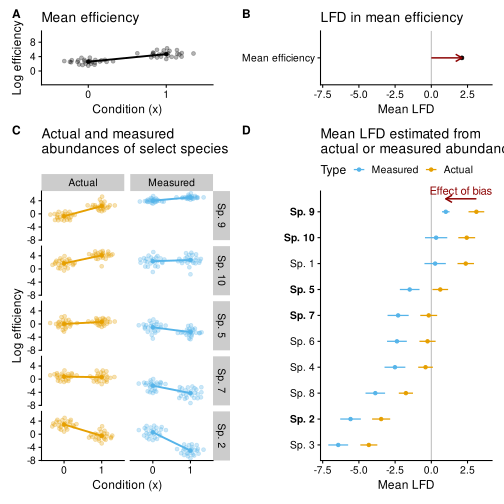
\includegraphics{figures/export-pdf/home/michael/research/differential-abundance-theory/notebook/_posts/2021-08-03-simulate-regression-example/simulate-regression-example_files/figure-html5/main-figure-1.pdf}
\caption{\label{fig:regression-example}\textbf{Taxonomic bias distorts multi-sample differential abundance inference when the mean efficiency of samples is associated with the covariate of interest.} This figure shows the results of a regression analysis of simulated microbiomes consisting of 50 samples and 10 species from two environmental conditions indexed by \(x=0\) and \(x=1\). In this simulation, the species with the largest efficiency (Species 9) also has the largest positive LFC, which drives the positive association of the log mean efficiency with the condition (shown in Panels A and B). This positive LFC in the log mean efficiency induces a systematic negative shift in the estimated LFCs of all species (Panels C and D). Panel D shows the mean LFC (points) with 95\% confidence intervals (CIs), for each species estimated from either the actual or the measured densities. The error (difference in LFC estimates on measured and actual) equals the negative LFC of the mean efficiency (shown in Panel B).}
\end{figure}



\hypertarget{implications}{%
\section{Implications for real-world inference~}\label{implications}}

Are biologically significant errors in DA analyses likely in practice?
We can begin to answer this question using a combination of theoretical analysis, consideration of hypothetical scenarios, and analysis of case studies for which some information about taxonomic bias is available.

\hypertarget{systematic-error-in-slope-or-lfc-estimates}{%
\subsection{Systematic error in slope or LFC estimates}\label{systematic-error-in-slope-or-lfc-estimates}}

Recall from Section \ref{differential-abundance} that the error in the slope or LFC in a DA regression analysis is proportional to the covariance of the log mean efficiency with the covariate.
This covariance can be split into two components: the standard deviation of (log) mean efficiency and its correlation with the covariate.
Hence when considering whether taxonomic bias creates large error, it can be useful to separately ask whether the mean efficiency is likely to vary across samples and whether it is likely to be correlated with a covariate of interest.

One approach to studying the mean efficiency empirically is to analyze data from studies for which control measurements allow direct measurement of species' efficiencies.
To characterize bias in a 16S sequencing protocol developed for the Vaginal Human Microbiome Project (VaHMP), Brooks et al. (\protect\hyperlink{ref-brooks2015thet}{2015}) performed 16S rRNA gene sequencing of mock communities of seven bacterial species thought to play a critical role in the human vaginal microbiome.
This protocol was later used for the VaHMP's Multi-Omic Microbiome Study: Pregnancy Initiative (MOMS-PI) study (Fettweis et al. (\protect\hyperlink{ref-fettweis2019thev}{2019})).
We used the method for measuring and correcting bias developed by McLaren, Willis, and Callahan (\protect\hyperlink{ref-mclaren2019cons}{2019}) to measure bias from the mock communities and analyze its potential impact on DA analyses that use the MOMSPI measurements (SI Analysis MOMS-PI).
The vaginal microbiome during pregnancy is characterized by relatively low diversity, with a single species often forming a vast majority of calibrated or uncalibrated read counts.
The three species that most often dominate the calibrated profiles are \emph{Gardnerella vaginalis}, \emph{Lactobacillus iners}, and \emph{Lactobacillus crispatus}.
Our mock-community analysis indicate \emph{G. vaginalis} has the lowest efficiency of the seven species, roughly 20X lower than \emph{L. crispatus} and 30X lower than \emph{L. iners} (the most efficiently measured).
As a result, the mean efficiency varies substantially across samples, with samples dominated by a \emph{Lactobacillus} species typically having an efficiency that is 3-20X greater than samples dominated by \emph{Gardnerella} (Figure \ref{fig:momspi-mean-efficiency-dist}).
Shifts between \emph{Lactobacillus} and \emph{Gardnerella} dominance are common in between-women comparisons, and also occasionally occur between subsequent sampling points in individual women (SI Figure \ref{fig:momspi-mean-efficiency-fcs}).
Examination of the multiplicative trajectories in the proportions of individual species indicates that such transitions can cause spurious fold changes in lower-abundance species (SI Figure TODO).
Decreases in mean efficiency during transitions from \emph{Lactobacillus} to \emph{Gardnerella} dominance can be expected to be even more extreme for commonly-used vaginal microbiome primers that fail to amplify \emph{Gardnerella}.

\begin{figure}
\centering
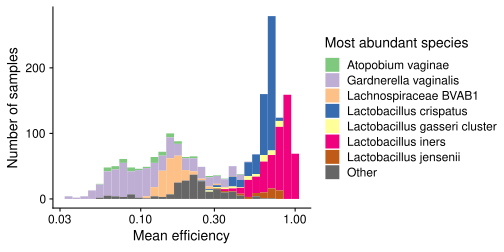
\includegraphics{figures/export-pdf/notebook/_posts/2021-11-01-momspi-summary/momspi-summary_files/figure-html5/momspi-mean-efficiency-dist-1.pdf}
\caption{\label{fig:momspi-mean-efficiency-dist}\textbf{The mean efficiency in vaginal samples from the MOMS-PI study varies with the most abundant species.}}
\end{figure}



A second study in which control communities make it possible to directly analyze the impact of taxonomic bias in experimental samples was performed by Leopold and Busby (\protect\hyperlink{ref-leopold2020host}{2020}).
To study the interactions between a host plant and its fungal commensals and pathogen, the authors inoculated trees with a fungal synthetic community and later exposed plants to a fungal pathogen.
The authors used ITS amplicon sequencing to measure communities before and after infection, along with mock communities which they used to estimate the species efficiencies with the method of McLaren, Willis, and Callahan (\protect\hyperlink{ref-mclaren2019cons}{2019}).
(DNA mocks were used, so that bias due to DNA extraction is not included, but other major bias sources such as PCR and ribosomal copy-number-variation are included.)
We reanalyzed this experiment to consider the impact that bias has on different possible DA analyses (SI Analysis Fungi).
As noted by Leopold and Busby (\protect\hyperlink{ref-leopold2020host}{2020}), there was a 13X difference between the most and least efficiently measured commensals, while the pathogen was measured 40X more efficiently than the least efficiently measured commensal.
Yet despite this 13X variation among commensals, the mean efficiency is remarkably stable across communities prior to pathogen colonization.
Consequently, taxonomic bias creates little systematic error in proportion-based DA analysis of these pre-colonization samples.
The high efficiency of the pathogen did, however, typically lead to a roughly 6X increase in the mean efficiency of post-colonization samples.
Hence DA analysis of how commensals responded to the pathogen did not first discard pathogen reads would therefore tend to suggest that the commensals had substantially smaller fold changes than they actually did, unless bias were accounted for.

It is clear that an individual species with an unusually high or low efficiency can drive large changes in the mean efficiency when it shifts from a very large (\(\sim 1\)) to very small proportion (\(\ll 1\)) of the sample.
Consideration of dynamics in the human gut illustrates another a way in which large shifts in higher-level taxa might create similar shifts, due to the fact that efficiencies do not vary independently among closely related species.
Gut microbiomes are dominated by two phyla: The Bacteroidetes and the Firmicutes, the ratio of which varies substantially across individuals.
Within a sample, there are usually multiple species contributing to the abundance of each phylum, with the median Inverse Simpson diversity being around 4 for each phylum in the HMP2 IBD study.
Thus changes from Bacteroidetes to Firmicutes dominance are unlikely to be driven by a single species.
However, if Firmicutes species tend to have systematically different efficiencies than Bacteroidetes species, then changes in phylum dominance can be expected to drive substantial changes in the mean efficiency even if many species contribute.
Indeed, several studies have found DNA extraction protocols to more efficiently lyse Gram-negative Bacteroidetes species than Gram-positive Firmicutes species (though substantial variation within phyla also occurs, McLaren, Willis, and Callahan (\protect\hyperlink{ref-mclaren2019cons}{2019})).

Systematic error in DA results requires that the variation in log mean efficiency is correlated with the covariate.
The examples above each suggest plausible biologically-significant scenarios in which such correlations might arise.
For example, in the vaginal microbiome a decline in \emph{Lactobacillus} and rise of species including \emph{Gardnerella vaginalis} is associated with preterm birth in pregnant women; hence the variation in mean efficiency driven by these species may also create an association of mean efficiency with preterm status.
In the plant-fungal experiment of Leopold and Busby (\protect\hyperlink{ref-leopold2020host}{2020}), the increase in pathogen proportion after infection leads to a large increase in the mean efficiency over time, which systematic increases the observed decline in the proportions of commensal species (SI Analysis).
The Bacteroidetes-to-Firmicutes ratio has also been linked to host conditions.
Yet in the HMP2 IBD dataset, the large variation in this ratio is largely independent of disease status, suggesting that the primary effect of any variation in mean efficiency driven by these phyla would be to increase noise rather than create systematic error in DA analysis.

Are there general mechanisms by which we might expect associations to arise between mean efficiency and the covariates commonly of interest in microbiome studies?
One possibility is that the ecology and measurement efficiency of species may become correlated simply due to shared evolutionary history.
A species' efficiency is heavily influenced by genetically determined traits such as cell-wall structure, ribosomal-operon copy number, sequence in a primer-targeted region, GC content, and even whether the species is present in a given taxonomic database.
Shared evolutionary history creates positive trait associations among more closely related species, such that we should expect a significant degree of phylogenetic conservation in efficiency.
Meanwhile, the same shared evolutionary history creates phylogenetic conservation in ecological traits that drives species abundance dynamics.
In this way, we may expect evolution to lead to a situation in which groups of species with similar efficiencies have similar shifts in abundance between conditions, creating the potential for commensurate shifts in mean efficiency.
For example, a change in diet that favors Bacteroidetes species relative to Firmicutes based on the resulting gut conditions will also increase the relative abundance of easy-to-lyse species.

Associations between efficiency and abundance can also arise more directly when a single microbial trait affects both.
For example, microbes at the ocean floor are slowly buried, sinking into a low nutrient, low oxygen environment.
Lloyd et al. (\protect\hyperlink{ref-lloyd2020evid}{2020}) estimate the log fold change in the estimated absolute abundance of various taxa with sediment depth (as a proxy for time) to determine which taxa are able to persist and even grow in this difficult environment.
It is plausible that microbes with tougher cell walls would tend to persist longer (alive or dead) in the sediment, while at the same time being more difficult to extract DNA from than microbes with weaker cell walls.
As the relative abundance of tougher species increases with depth, the mean extraction efficiency might therefore decrease.
This decrease would increase the inferred log fold changes and could lead to inferred growth of taxa that are actually just persisting or even slowly dying off.
Additional measurements by Lloyd et al. (\protect\hyperlink{ref-lloyd2020evid}{2020}) make it possible to investigate this possibility explicitly.
The primary analysis, which used proportion-based density estimates, was supported by targeted measurements (qPCR) of 16S concentration for particular taxa.
For instance, in Core 30, the doubling time estimated for the Archaeal phylum Bathyarchaeota was estimated to be 10.1 years using the proportion-based densities and 10.3 years by qPCR (Lloyd et al. (\protect\hyperlink{ref-lloyd2020evid}{2020}) Table 1 and Figure 4).
These doubling times correspond to highly similar estimated slopes of log density per year of \(1/10.1 \approx 0.99\) and \(1/10.3\approx 0.97\).
The small difference between these slopes suggests that there is little correlation of log mean efficiency with burial time and hence little systematic error in the estimated doubling times derived from the proportion-based density estimates.

Another example of a trait that might simultaneously affect efficiency and relative abundance is ribosomal copy number, which increases the measurement efficiency in ribosomal amplicon experiments and is also linked to differences in ecology and population dynamics among species.

The biological significance of the error in \(\hat \beta\) depends on the relative magnitude of the LFC (or covariance with the covariate \(x\)) in the focal species vs in the mean efficiency.
It may generally be true that the largest species LFCs in a DA analysis, which are often of primary interest in a microbiome study, will tend to be larger than the LFC of the mean efficiency, at least in high-diversity settings.
Further investigation into this question may improve our confidence in the top hits identified in published DA analyses meeting certain conditions.
However, we must remain weary of cases (as in the vaginal-microbiome and plant-fungal-interactions examples above) in which a shift in a single species can drive large changes in mean efficiency and lead to significant errors for other species.
The experimental and computational methods discussed in Section \ref{solutions} can mitigate taxonomic bias in these clearly-problematic cases while also helping to amass empirical evidence on the conditions in which bias is unlikely to cause major inferential errors.

\hypertarget{loss-of-precision-and-power}{%
\subsection{Loss of precision and power}\label{loss-of-precision-and-power}}

Another way in which taxonomic bias hinders DA analysis is by increasing the noise in abundance measurements, leading to a reduction in the precision of LFC estimates and thus the power to detect true associations.

There are two distinct mechanisms by which such reductions occur.
The first was described in Section \ref{differential-abundance}: Variation in the mean efficiency that is random (in the sense of being unassociated with the covariates in a regression analysis) tends to increase the standard errors in estimated regression coefficients.
As noted above, this effect may be the dominant one in cases like the HMP2 IBD dataset where large variation in dominant phylum is independent of disease status.
Correcting for the variation in mean efficiency using the calibration methods described in the next section can reverse this effect, thereby increasing the precision as well reducing the systematic error in DA inference.

The second mechanism involves the counting noise that stems from the random sampling of reads in the sequencing experiment.
This counting noise is expected to be the dominant source of noise for species whose expected proportion \emph{after accounting for taxonomic bias} is \(\lesssim 1 / \text{total reads}\) for a given sample.
Having an atypically low efficiency makes a species much more likely to be near this threshold and hence to receive highly uncertain measurements.
Such imprecise measurements can make it near impossible to make biologically meaningful conclusions.
For example, in the experiment of Leopold and Busby (\protect\hyperlink{ref-leopold2020host}{2020}) described above, the median read counts in samples taken after pathogen colonization for the 5 commensals with the lowest efficiencies were 0, 0, 0, 1, and 11.
These species' efficiencies ranged from 40X-10X lower than the pathogen's efficiency; thus, in the absence of bias the counts may have been much higher and it might have been possible to make much more precise conclusions about how their relative abundances changed during pathogen invasion.
The literature on the vaginal microbiome during pregnancy provides us with another example: Disagreement among studies over whether \emph{Gardnerella} is positively associated with preterm birth seems to be in part driven by the fact that several studies used 16S primers that are extremely poor at amplifying \emph{Gardnerella} and hence lack the precision necessary to find associations even were they to exist.
Unfortunately, even perfect knowledge of the measurement efficiencies will not allow us to overcome the low precision caused by small expected read counts; however, the methods described in the section provide principled ways to assess whether the low counts are due to taxonomic bias rather than truly low frequencies in a species' abundance.

\hypertarget{solutions}{%
\section{Potential solutions}\label{solutions}}

The theoretical results from Section \ref{differential-abundance} suggest a number of potential methods to avoid, correct, or otherwise mitigate the errors created by taxonomic bias.

\hypertarget{analyses-of-fold-changes-in-species-ratios}{%
\subsection{Analyses of fold changes in species ratios}\label{analyses-of-fold-changes-in-species-ratios}}

Since the fold changes in species ratios are unaffected by consistent taxonomic bias, a natural approach to countering bias in relative DA analysis is to ratio- rather than proportion-based methods.
A variety of such methods have been developed for microbiome DA analysis that build on earlier work from the field of Compositional Data Analysis (CoDA).
These methods analyze log-fold changes in the ratios among a pair of species or, more generally, some product of exponential power of multiple species, which likewise are bias-invariant.
Besides a greater robustness to taxonomic bias, such ratio-based analyses have other advantages.
First, analysis of ratios avoids other standard criticisms leveled at proportion-based analysis---namely that the change in proportion of a species is affected by change in the density of all other species and the set of species used in the denominator of the proportion calculation (Gloor et al. (\protect\hyperlink{ref-gloor2017micr}{2017})).
Second, ratios may be more informative than absolute density in some cases, such as for swabs or other sample types for which the absolute density in the sample may be an unreliable indicator of the absolute density of the sampled ecosystem.

Ratios come with their limitations, however.
First, there are a vast number of species ratios (and derivatives) to potentially consider, none of which provide direct information about absolute densities, which can make choosing and interpreting a ratio-based DA analysis challenging.
Second, ratio measurements are impacted by noise in both the numerator and denominator and so can be noisier than proportion measurements, particularly when the read counts in the denominator are small.
A related problem is that, due to the discrete nature of biological organisms and the reads that are generated during sequencing, species in the denominator are commonly observed to have 0 reads; the assumptions that made by different methods about the meaning of these 0 counts can have a major impact on DA results.
Finally, bias invariance at the level of ratios among species does not extend to ratios of additive aggregates of species, such as between bacterial phyla, unless further conditions are met (McLaren, Willis, and Callahan (\protect\hyperlink{ref-mclaren2019cons}{2019})).

\hypertarget{calibrate-compositions}{%
\subsection{Calibration using community controls}\label{calibrate-compositions}}

Measurement of community calibration controls along with the primary experimental samples can enable researchers to directly measure and remove the effect of bias prior to or concurrent with downstream DA analysis.
Community calibration controls are samples whose species identities and relative abundances are known either by construction or by characterization with a chosen `gold standard' or \emph{reference protocol} (McLaren, Willis, and Callahan (\protect\hyperlink{ref-mclaren2019cons}{2019})).
MGS measurement of one or more control communities can be used to directly measure the relative efficiencies among the superset of species in the controls (McLaren, Willis, and Callahan (\protect\hyperlink{ref-mclaren2019cons}{2019})).
The measured relative efficiencies can then be used to calibrate (remove the effect of bias from) the relative abundances (ratios) of the control species in a set of primary (non-control) experimental samples that were measured with the same protocol (ideally in the same experiment and sequencing run) (McLaren, Willis, and Callahan (\protect\hyperlink{ref-mclaren2019cons}{2019})).
Calibration can be extended to species not in the controls using statistical methods to impute (predict) the unobserved efficiencies using phylogenetic relatedness, genetic characteristics (such as 16S copy number), and/or phenotypic properties (such as cell-wall structure).

The calibrated compositions can be used for arbitrary downstream microbiome analyses, including relative and absolute DA analysis.
To demonstrate the potential for calibration to improve fold-change measurements, we estimated bias from one sample in the mock community data from Brooks et al. (\protect\hyperlink{ref-brooks2015thet}{2015}) that contained all 7 species and used it to calibrate the compositions of all samples (Figure \ref{fig:calibration-example}).
We then estimated species' densities using the uncalibrated and calibrated proportions using the community normalization method, treating the total density as known and fixed.
Visual inspection shows that the bias estimated from just a single control community with all species can be sufficient to greatly reduce the effect of taxonomic bias on the measured fold change in species' proportions and densities (Figure \ref{fig:calibration-example}).
To demonstrate a practical application, we used the bias estimated from the full set of mock communities as the basis for calibrating the vaginal community time series measurements from the MOMS-PI study (Fettweis et al. (\protect\hyperlink{ref-fettweis2019thev}{2019})) that were made using the same 16S sequencing protocol.
We imputed the efficiencies of other species using taxonomic relationships (Methods).
Calibration then allowed us to explore the impact of bias on the measured trajectories of species proportions within women over the course of pregnancy as described in Section \ref{implications}.

\begin{figure}
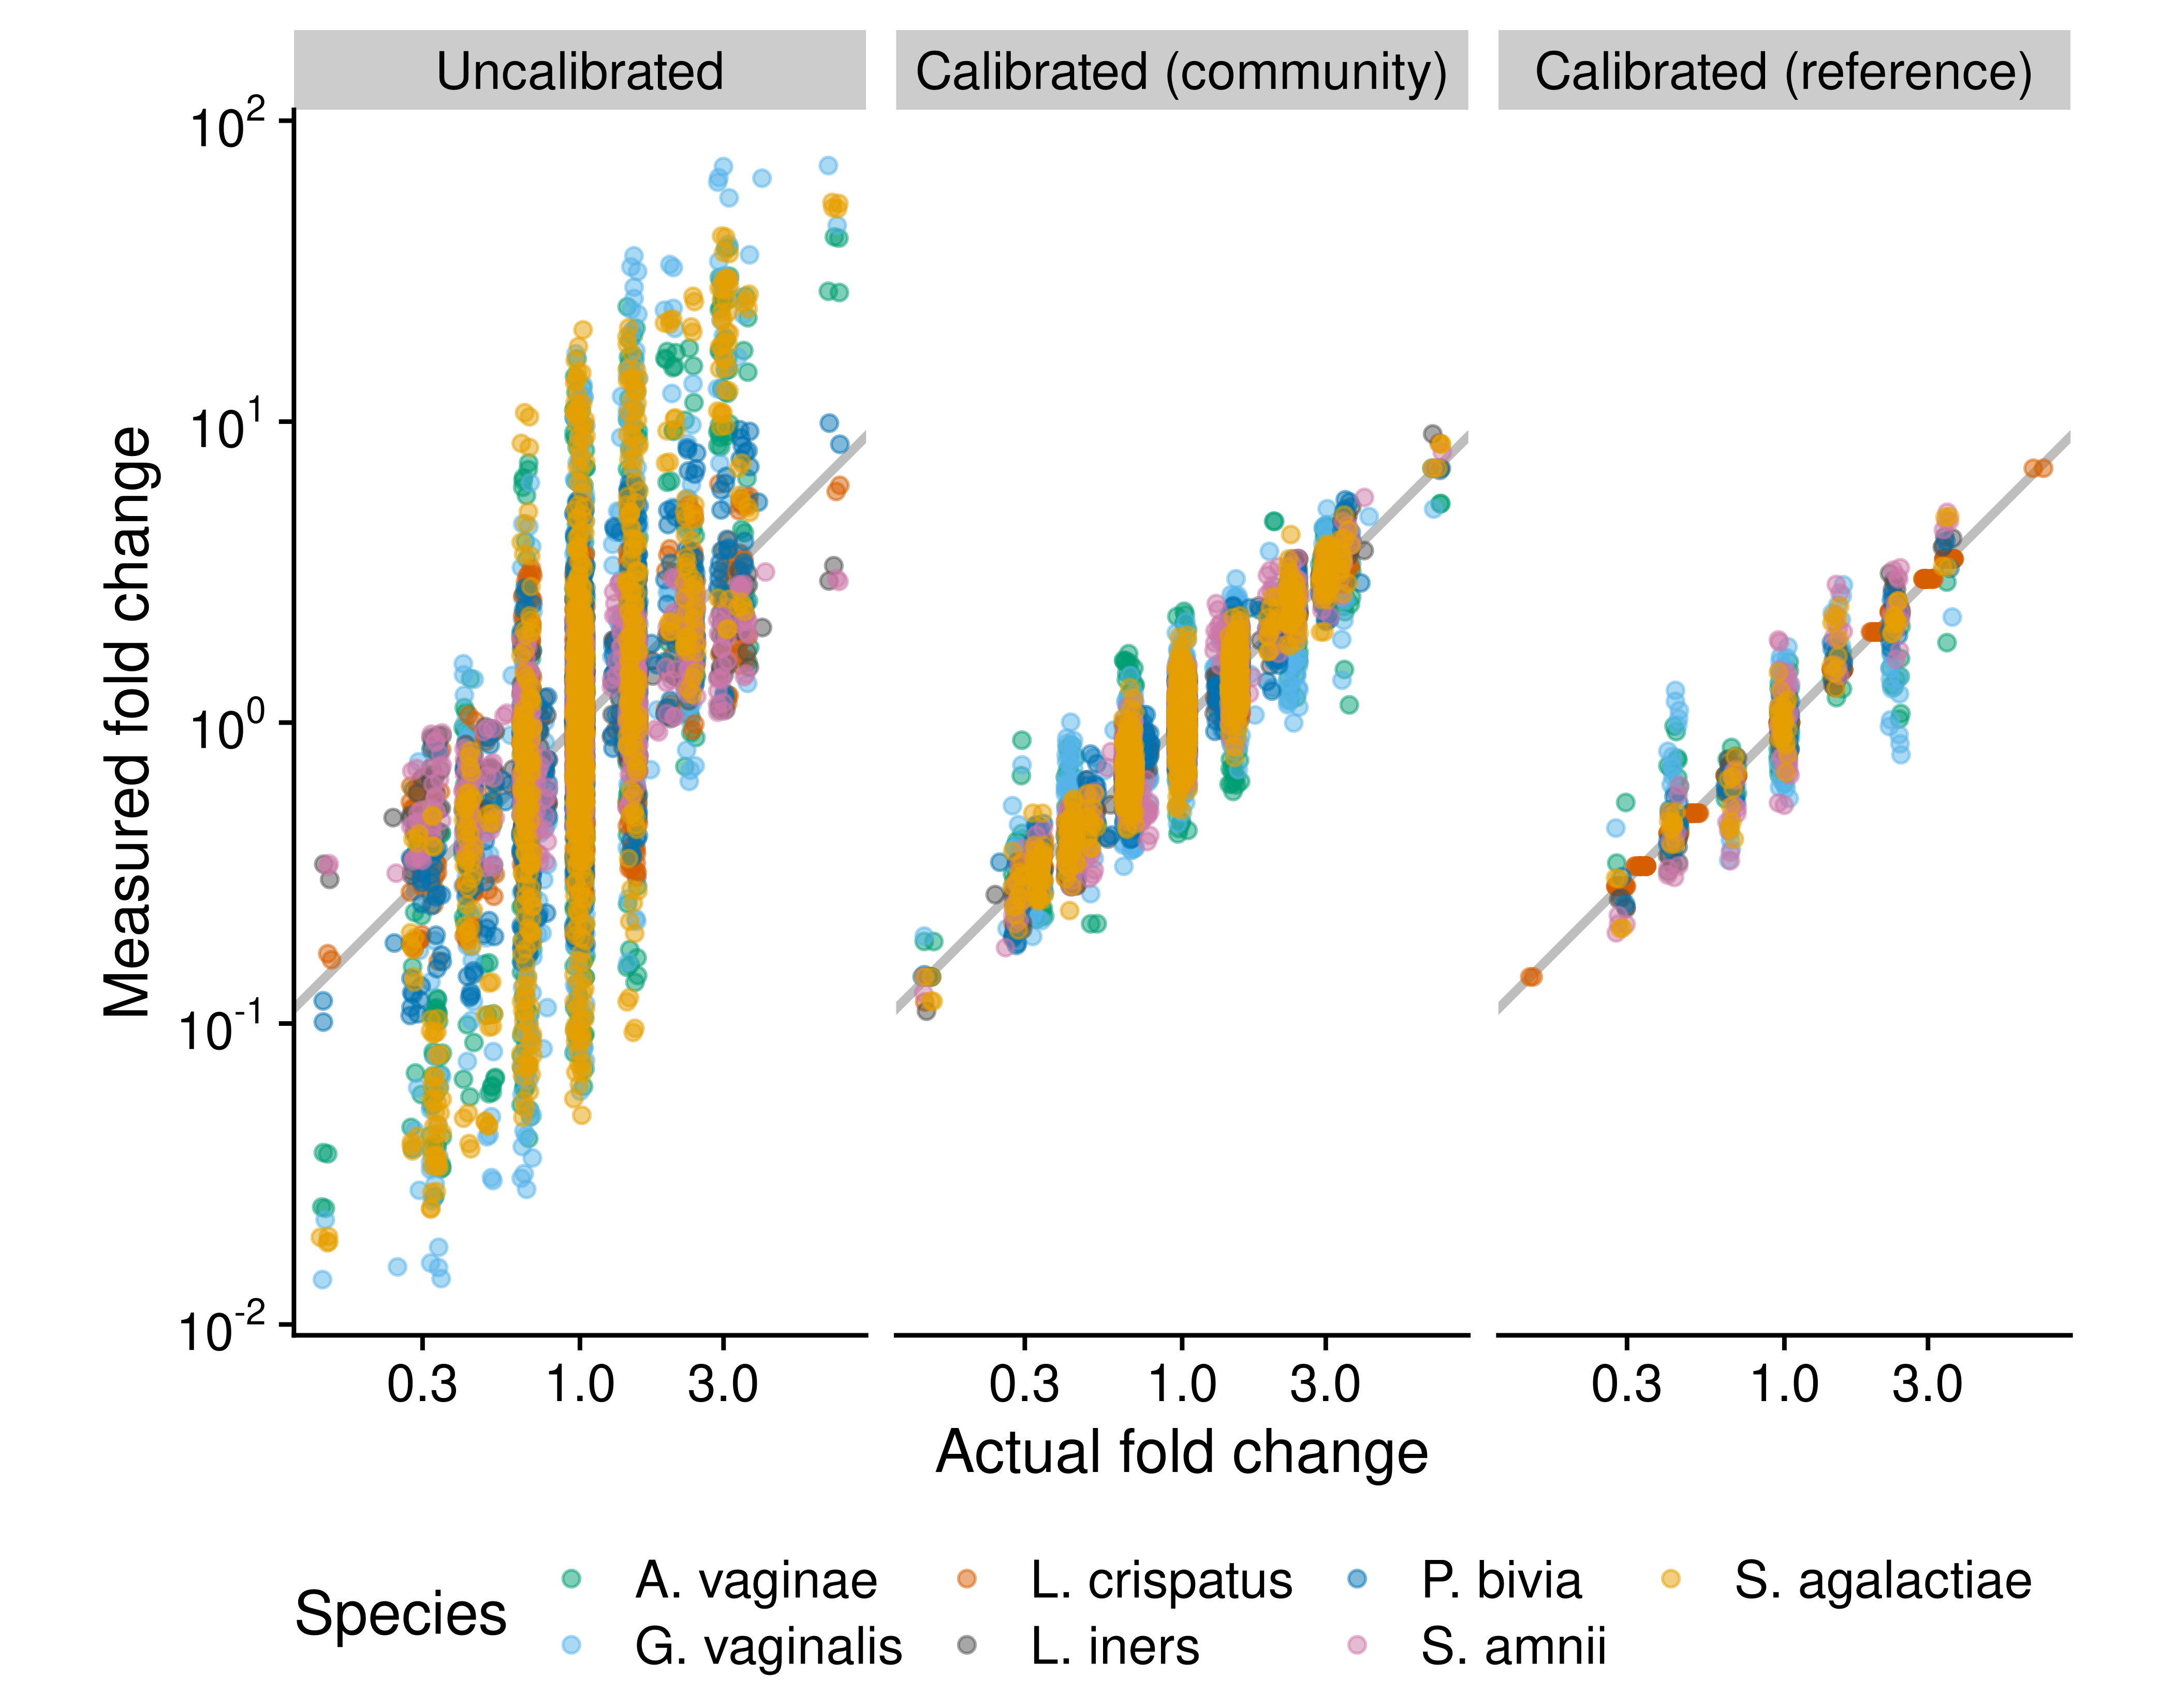
\includegraphics[width=1\linewidth]{notebook/_posts/2021-10-25-brooks2015thet-calibration/brooks2015thet-calibration_files/figure-html5/brooks2015thet_fc_calibration-1} \caption{\textbf{Fold changes can be calibrated using community controls or reference species.} The figure compares the performance of three methods for measuring fold changes in absolute cell density in cellular mock communities of 7 vaginal species, which were constructed and measured via 16S sequencing by Brooks et al. (\protect\hyperlink{ref-brooks2015thet}{2015}). The `Uncalibrated' fold changes are derived directly from uncalibrated individual abundance measurements, which equal the product of the species' proportion by the total density (which here is be known to be constant by construction). The `Calibrated (community)' measurements are computed from abundance measurements where the proportions are first corrected for the taxonomic bias that was estimated from a single sample that contained all 7 species. The `Calibrated (reference)' measurements are computed from abundances measured with the reference-species method, with \emph{Lactobacillus crispatus} used as the reference; that is, the true abundance of \emph{L. crispatus} is treated as known and used to infer the abundance of the remaining 6 species. Only samples that contain \emph{L. crispatus} are included.}\label{fig:calibration-example}
\end{figure}



\hypertarget{calibration-using-reference-species}{%
\subsection{Calibration using reference species}\label{calibration-using-reference-species}}

Obtaining control communities that span the taxa of interest is often not practical.
Moreover, the bias that is measured from controls may differ from that in the primary samples due to differences in cell state or sample preparation.
These problems may be overcome for the purpose of species-level absolute DA analysis by using the reference-species approach to absolute-density measurement that was described in Section \ref{differential-abundance}.
This \emph{reference-species calibration} allows one to simultaneously account for changes in total density and the sample mean efficiency, obtaining accurate fold changes in absolute density from taxonomically biased, relative metagenomics measurements.

Recall that densities estimated by the reference-species approach have a constant fold error, provided that the fold error in the reference species is also constant (Equation \eqref{eq:density-ratio-error}).
Three categories of reference species are reviewed for this purpose in Appendix \ref{review-absolute-methods}, including why they might be expected to produce constant fold errors: housekeeping species assumed to have constant abundance, spike-in species added at known or constant abundance, and species whose abundance has been measured with a targeted method like species-specific qPCR.

To demonstrate the ability for reference calibration to improve fold changes, we treated the abundance of one species (\emph{Lactobacillus crispatus}) in the Brooks et al. (\protect\hyperlink{ref-brooks2015thet}{2015}) mock community data as known, and used it to calibrate the abundances of all species.
Doing so improved the resulting measurements of fold changes in density for all species (Figure \ref{fig:calibration-example}).

\hypertarget{choosing-complementary-total-density-and-metagenomics-measurements}{%
\subsection{Choosing complementary total-density and metagenomics measurements}\label{choosing-complementary-total-density-and-metagenomics-measurements}}

A variety of methods for measuring total community density have been paired with either amplicon or shotgun sequencing data for the purpose of conducting absolute DA analysis using the total-density approach described in Section \ref{differential-abundance}.
Each of these methods is subject to its own taxonomic bias: Cells from different species are likely to contribute more or less efficiently to the total abundance measurement.
Consider the popular method of assessing bacterial abundance with total-16S qPCR measurement.
Even an ideal qPCR protocol that perfectly amplifies all species remains a biased measurement of cell density, since the total 16S copies in the extracted DNA contributed by each species will be proportional to its (species-specific) lysis efficiency and 16S copy-number.
16S qPCR is commonly paired with 16S amplicon sequencing, with which these sources of bias are shared, perhaps along with variation in primer binding and amplification efficiency.
Methods like using flow cytometry that directly measures cell density lacks these biases but likely have their own that are more likely to be orthogonal to the 16S sequencing measurement.
By extending the analysis of Section \ref{differential-abundance} to include consistent taxonomic bias in the total-density measurement, we find that pairings of total-density and sequencing measurements that share large sources of taxonomic bias can lead to an offsetting of errors that reduces the error in fold-change measurement and DA inference (Appendix \ref{total-density-bias}).
This finding suggests that methods of total-density measurement that are more accurate as measures of total cell density may actually perform worse than less accurate methods for the purposes of absolute DA inference.

We illustrate with a hypothetical example of two vaginal communities of equal density, but which are dominated either by \emph{Lactobacillus iners} or \emph{Gardnerella vaginalis}.
Based on our earlier analysis in McLaren, Willis, and Callahan (\protect\hyperlink{ref-mclaren2019cons}{2019}), we estimate that \emph{L. iners} yields 10X more 16S copies per cell than \emph{G. vaginalis} in extracted DNA.
Ignoring other sources of bias, we expect relative efficiencies of \emph{L. iners}:\emph{G. vaginalis} of 10 for both qPCR and 16S sequencing measurements.
Consequently, the \emph{G. vaginalis} community will yield a substantially lower qPCR measurement than the \emph{L. iners} community and we would incorrectly infer a decrease in total abundance.
At the same time, this decrease in the mean efficiency of the sequencing measurement would cause artificially high fold changes in the proportions of all species (Section \ref{differential-abundance}).
When using qPCR and 16S sequencing measurements for community-based density estimation, these two opposing errors cancel, yielding accurate fold changes in species densities.

More generally, changes in the mean efficiency of the total density measurement offset those in the sequencing measurement when comparing log density of species across samples.
If the (log) efficiencies of the total and sequencing measurement are positively correlated across species, then the (log) mean efficiencies will tend to be positively correlated across samples, leading to a reduction in error in DA analysis relative to total-density methods whose efficiencies are uncorrelated with those of the sequencing measurement.
These observations suggest that qPCR of a marker gene may be the ideal pairing for amplicon sequencing measurements, despite being a poor measure of changes in total cell density.
Similarly, bulk DNA quantification may be an ideal pairing for shotgun sequencing, making it possible to account for variation in lysis efficiency and genome length.
These pairings even make it possible to account for error caused by variation among samples in the fraction of unclassified reads, which can form a major fraction of amplicon and shotgun data.
Importantly, maximizing the offsetting of errors requires thoughtful choices during bioinformatic analysis, perhaps eschewing the filtering and normalization steps used in many software packages and workflows (Appendix \ref{total-density-bias}).

\hypertarget{bias-sensitivity-analysis}{%
\subsection{Bias-sensitivity analysis}\label{bias-sensitivity-analysis}}

For experiments that have been conducted without calibration controls, it is still possible to investigate the likelihood that DA results can be explained by taxonomic bias by performing a computational bias-sensitivity analysis.

A bias-sensitivity analysis examines how sensitive the results of a given DA analysis are to the working assumption about the bias of a given protocol.
This working assumption is typically is that there is no bias, but could also be bias measured in a previous experiment or predicted from taxonomic features like 16S copy number.
A straightforward approach to bias-sensitivity analysis is to use computer simulation to re-analyze the MGS data across a set of simulated taxonomic biases.
First, multiple sets of efficiency vectors are randomly generated, each representing a possible quantification of taxonomic bias for the study.
Second, each efficiency vector is used to calibrate the original MGS measurements; each set of calibrated measurements represents the true community compositions under the given hypothesized bias.
Finally, the DA analysis is re-run on each set of calibrated measurements and the distribution of results is compared graphically or with summary statistics.
A graphical summary of such an analysis being applied to results from the corncob frequentist DA- analysis tool `corncob' are shown in SI Figure \ref{fig:sensitivity-example}.
The simulated efficiency vectors may be generated to different hypotheses about bias in the given system, such as its overall magnitude and correlation among phylogenetically-related species.
Thus the utility of such simulations will increase the more we learn about the properties of taxonomic bias in different systems.

An alternative approach to bias-sensitivity analysis would be to directly include the (unknown) taxonomic bias of the protocol in the statistical model used for DA analysis, as described for bias-aware meta-analysis below.
Further development of tools and workflows for performing bias sensitivity analyses could be a valuable way to assay and improve the reliability of microbiome results---for differential abundance and microbiome analyses more generally.

\hypertarget{bias-aware-meta-analysis}{%
\subsection{Bias-aware meta-analysis}\label{bias-aware-meta-analysis}}

So far we have considered analysis of samples subject to the same taxonomic bias;
however, meta-analysis of microbiome samples measured across multiple studies must often contend with a diversity of protocols and hence taxonomic biases in samples from different studies.
This inconsistency in taxonomic bias across studies poses a problem even for ratio-based analyses.
A potential solution is to perform a bias-aware meta-analysis that that explicitly accounts for the possibility of distinct taxonomic bias across studies.

Parametric microbiome meta-analysis models include sets of species-specific latent parameters to model ``batch effects''---amorphous differences in the measurements of each study.
By configuring these models so that these latent parameters correspond to study-specific species efficiencies, we can improve their biological interpretability and gain the ability to directly assess whether disagreements in DA results across studies can be explained by differences in taxonomic bias.
To the extent that taxonomic bias truly is consistent within studies, meta-analyses that directly account for it can have greater statistical power to extract the truly consistent and inconsistent microbial patterns across studies.

\hypertarget{appendix-appendix}{%
\appendix \addcontentsline{toc}{section}{\appendixname}}


\hypertarget{model-details}{%
\section{Model details}\label{model-details}}

This appendix provides a more detailed description of our deterministic model of the microbiome measurement process, which it uses to derive some of the additional claims of the main text.

\hypertarget{mgs-measurement}{%
\subsection{MGS measurement}\label{mgs-measurement}}

This section expands the description of the model in the main text to more explicitly lay out our assumptions and to consider the effect of variation in measurement efficiencies within a taxonomic group on its MGS measurement.

A taxon can be any group of organisms.
For any taxon \(I\) and sample \(a\), we define the absolute efficiency of that taxon and that sample as the number of reads assigned to that taxon divided by the number of cells of that taxon in the given sample.
We assume that these assigned reads really do come from that particular taxon and sample (though this assumption is often violated in practice).

The efficiency of a taxon \(I\) is the average number of reads produced by each of its constituent cells.
This number varies due to

\begin{enumerate}
\def\labelenumi{\arabic{enumi}.}
\tightlist
\item
  Genetic variation among cells
\item
  Non-genetic variation among cells
\item
  Randomness in the experimental process
\end{enumerate}

Variation encoded in the genome of cells determines properties that affect its efficiency, such as how easy it is to lyse, how easily PCR primers will bind to their target locus, how many copies of a marker gene are in the genome, and whether its sequencing reads can be taxonomically assigned.
This variation created by genetically encoded traits is what we refer to as `taxonomic bias' and is the primary focus of this article.
In principle, even a single nucleotide change (e.g.~in a primer-binding site) could affect the efficiency of a cell.
Nevertheless, cells will more similar genomes will tend to have more similar genetically-encoded efficiencies.
For the purposes of our analysis, we suppose that cells within the same species have approximately identical genetically-encoded efficiencies.
The impact of violations in this assumption can be understood using the approach we describe below for taxa above the species level.
More generally, our results can be read as applying to the finest taxonomic unit that is reported by the given MGS method.

Genetically identical cells can differ in cell state such that their efficiencies vary significantly.
An extreme example is the effect of sporulation: Spores are generally harder to lyse than vegetative cells, and VanInsberghe et al. (\protect\hyperlink{ref-vaninsberghe2020diar}{2020}) found that the efficiency of a common DNA extraction protocol was 800X on vegetative cells vs spores of a strain of \emph{Clostridium difficile}.
Physiological differences might also arise simply due where they are in the cell cycle.
To the extent that the cells of a given genotype tend to have a similar distribution of cell states across samples, the efficiency of the genotype will remain stable.
We assume this stability throughout our analysis.
Violations in this assumption can again be understood using an approach similar to that we use to considering taxa above the species level.

The final number of reads also varies due to idiosyncratic events that we typically think of (and model) as `random', such as the precise handling of a sample during pipetting or loading of a sequencing flow cell.
Such variation may or may not be dwarfed by the `random' variation in the sample composition (i.e., the variation not explained by the covariates in a regression analysis).
For simplicity, we ignore this random variation when considering the impact of taxonomic bias on MGS measurement.
The effect of random variation in regression analysis is addressed in Appendix
\ref{appendix-regression} and the effect of random counting error is discussed in Section \ref{implications}.

The absolute efficiency of a taxon can also vary simply because more effort is put towards sequencing that sample, either intentionally or unintentionally.
The sequencing effort might depend on the taxonomic composition and bias of a sample.
For example, a sample with higher output DNA will often be diluted more prior to amplification or sequencing.
The critical assumption we make regarding sequencing effort is that it affects all species in the sample equally and hence doesn't affect their relative abundances.

With these assumptions in place, we can partition the multiplicative difference between the reads assigned to a taxon and its density in the source sample into a taxon-specific factor and a sample-specific factor.
There is an extra degree of freedom, which we settle by equating the taxon-specific factors with relative measurement efficiencies and arbitrarily choose the relative efficiency of a particular species to equal 1.

Our model for the read counts of a species \(i\) in sample \(a\) can thus be expressed mathematically as
\begin{align}
  \text{reads}_{i}(a)
  = \text{density}_{i}(a) \cdot \text{efficiency}_{i} \cdot \text{effort}(a).
\end{align}
Note that the species' efficiencies are properties of the species \(i\) but not the sample \(a\).
Similarly, let \(\text{density}_{I}(a)\), \(\text{reads}_{I}(a)\), and \(\text{efficiency}_{I}(a)\) denote the density, read count, and relative efficiency of an arbitrary group of species \(I\) in sample \(a\).
The read count for taxon \(I\) in sample \(a\) can be written
\begin{align}
  \label{eq:measurement-model-general}
  \text{reads}_{I}(a)
  = \text{density}_{I}(a) \cdot \text{efficiency}_{I}(a) \cdot \text{effort}(a).
\end{align}
The efficiency of taxon \(I\) in sample \(a\) equals the weighted average of its constituent species,
\begin{align}
  \label{eq:efficiency-general}
  \text{efficiency}_I(a) 
  \equiv \frac{\sum_{i\in I}\text{density}_i(a)\cdot \text{efficiency}_i}{\text{density}_I(a)}.
\end{align}
The ratio between the read counts of two taxa \(I\) and \(J\) is
\begin{align}
  \label{eq:ratio-error-general}
  \widehat{\text{ratio}}_{I/J}(a)
  &= \frac{\text{density}_{I}(a)}{\text{density}_{J}(a)} \cdot \frac{\text{efficiency}_{I}(a)}{\text{efficiency}_{J}(a)}.
\end{align}
Equation \eqref{eq:prop-error} for the error in a species' proportion and Equation \eqref{eq:ratio-error} for the error in the ratio between two species both follow directly from this more general expression.

\hypertarget{revised-main-text-equations}{%
\subsubsection{Revised main text equations}\label{revised-main-text-equations}}

Let \(S\) be the set of all species.
Then
\begin{align}
  \text{reads}_S(a)
    = \text{density}_S(a) \cdot \text{efficiency}_S(a) \cdot \text{effort}(a),
\end{align}
where
\begin{align}
  \text{efficiency}_S(a) 
  \equiv \frac{\sum_{j\in S}\text{density}_j(a)\cdot \text{efficiency}_j}{\text{density}_S(a)}
\end{align}
Also,
\begin{align}
  \widehat{\text{prop}}_{i}(a) = \frac{\text{reads}_i(a)}{\text{reads}_S(a)}.
\end{align}
and
\begin{align}
  \widehat{\text{prop}}_{i}(a)
  &= \text{prop}_{i}(a) \cdot \frac{\text{efficiency}_{i}}{\text{efficiency}_S(a)}.
\end{align}

\hypertarget{total-density-bias}{%
\subsection{Taxonomic bias in total-density measurement}\label{total-density-bias}}

To understand the impact of taxonomic bias in the total-density measurement on community normalization, we model error in total-density measurements similarly to that for MGS measurements.
Let \(\widehat{\text{density}}_{S}(a)\) be the measurement of the density of all species \(S\).
We suppose that this number is the sum of the (unobserved) contributions from each species.
The contribution of a species \(i\) is proportional to its actual density \(\text{density}_{i}(a)\) and its \emph{absolute efficiency for the total-density measurement} \(\text{efficiency}_{i}^{\text{tot}}(a)\).
The contributions may also be multiplied by a common sample-specific error factor to account for non-linearity of extraction and/or random error, which we ignore for now.
The measured total density therefore equals
\begin{align}
  \widehat{\text{density}}_S(a) 
  &= \sum_{i\in S} \text{density}_i(a) \cdot \text{efficiency}^{\text{tot}}_i
\\&= \text{density}_S(a) \cdot \text{efficiency}^{\text{tot}}_S(a)
\end{align}
where
\begin{align}
  \label{eq:app-total-mean-efficiency}
  \text{efficiency}^{\text{tot}}_S(a) 
  \equiv \frac{\sum_{i \in S}\text{density}_j(a)\cdot \text{efficiency}^{\text{tot}}_i}{\text{density}_S(a)}
\end{align}
is the mean efficiency in the sample with respect to the total-density measurement.

The error in the total density depends on the species composition through the mean efficiency of the sample; hence spurious changes in measured density can occur simply due to shifts from high- to low-efficiency species (or vice versa).

How does this error affect the measured densities of individual species when the total is used for normalization?
Substituting the mean efficiency of the total measurement for the error term in Equation \eqref{eq:density-prop-error} gives
\begin{align}
  \label{eq:app-density-prop-error}
  \widehat{\text{density}}_{i}(a) 
  = \text{density}_{i}(a) \cdot \frac{\text{efficiency}_{i} \cdot \text{efficiency}^{\text{tot}}_S(a)}{\text{efficiency}_S(a)}.
\end{align}
The mean efficiency of the total measurement appears in the numerator, while the mean efficiency of the MGS measurement is in the denominator.
To the extent that these two are positively associated across samples (specifically, their logarithms are positively linearly correlated), then the variation in one will tend to be offset by the variation in the other.
In this case the (geometric) variation in the ratio will be reduced, and the fold error in the species density measurement will tend to be more consistent than if the total density measurement was taxonomically unbiased (i.e.~\(\text{efficiency}^\text{tot}_S(a) = 1\) for all samples).
The error in species densities for individual samples may not be reduced; but the error in fold changes and regression analysis across samples will be.

The extent to which the log mean efficiency of the MGS measurement and the total measurement are correlated depends on the species efficiencies as well as the changes in species composition across samples, making it difficult to make general statements about this effect.
We can get a sense for the effect by considering the correlation between log efficiencies across species between the two measurement types.
Suppose that distribution over species of log efficiencies of the MGS measurement has variance \(\sigma^{2}\), the log efficiencies for the total density measurement has variance \(\sigma_{\text{tot}}^{2}\), and the correlation between the two is \(\rho\).
The variance in the difference \(\log \text{efficiency}_{i}^{\text{tot}} - \log \text{efficiency}_{i}\) is thus \(\sigma^{2} + \sigma_{\text{tot}}^{2} - \rho \sigma \sigma_{\text{tot}}\).
All else equal, the smaller this variance, the smaller we expect the variation in the error factor \(\text{efficiency}^{\text{tot}}_S(a)/ \text{efficiency}_S(a)\).

\textbf{Unclassified reads:} It is common that a given MGS protocol generates sequencing reads from particular taxa that the bioinformatics portion entirely discards, due to an inability to taxonomically assign the reads to the chosen taxonomic units.
For instance, 16S data that is analyzed with closed-reference OTU assignment and shotgun data analyzed by mapping to a database of reference genomes will be unable to assign sequences that are less than a chosen similarity cutoff (e.g.~97\%) from the reference sequences.
These taxa may form an appreciable fraction of the community and thus lead to a large fraction of the total sequenced reads for a given sample may remain unassigned.

So far, we have defined the efficiency of the MGS protocol in terms of taxonomically classified reads and so have treated such taxa as having an MGS efficiency of 0.
If such species are included in the total density measurement, then we have a mismatch between the two measurement types.
However, we may be able to remove this mismatch by altering the equation we use to form species density measurements.
In particular, we can compute the proportion of the focal species from the ratio of its assigned reads to the total sequenced reads, rather than to the total set of assigned reads.
This approach raises additional questions around how to treat reads from assignable species that are filtered during quality control steps.

Suppose that the set of species that can be classified by our bioinformatics pipeline, \(S\), is a proper subset of a larger set of species \(S'\) that are present and yield sequencing reads in our sample.
Suppose that there is no additional taxonomic bias in our MGS measurement; that is, all species in \(S\) have an efficiency of 1, and the species in \(S' \setminus S\) have an efficiency of 0.
Moreover, suppose that all reads from the \(S\) species are classified; that is, there is no loss of reads due to routine QC filtering.
Further suppose that we are capable of perfectly measuring the total density of all cells from the full set of species \(S'\); that is, \(\text{efficiency}^{\text{tot}}_{i} = 1\) for all species \(i \in S'\).

In this case, we can overcome the mismatch between MGS and total measurement when we use them to measure species densities, by using the total reads rather than the assigned reads to compute the species proportions.
That is, instead of
\begin{align}
  \widehat{\text{prop}}_{i}(a) = \frac{\text{reads}_i(a)}{\text{reads}_S(a)},
\end{align}
we take
\begin{align}
  \widehat{\text{prop}}_{i}(a) 
  &= \frac{\text{reads}_i(a)}{\text{total reads}(a)}
\\&= \frac{\text{reads}_i(a)}{\text{reads}_{S'}(a)}.
\end{align}
By accounting for the contribution of unknown species when computing proportions, we are able to resolve the mismatch and obtain accurate species densities.

\hypertarget{total-density-ref}{%
\subsection{Using reference species for total-density normalization}\label{total-density-ref}}

Constant reference species are sometimes used to measure total density of \(S\) by the ratio of \(S\) reads to \(R\) reads.
For example, a study of \emph{Arabidopsis} microbiomes used the ratio of bacterial to host reads in shotgun sequencing as a proxy for total bacterial density, which they then used for total-community normalization of 16S amplicon sequencing measurements (Karasov et al. (\protect\hyperlink{ref-karasov2020ther}{2020}), Regalado et al. (\protect\hyperlink{ref-regalado2019comb}{2020})).
Chng et al. (\protect\hyperlink{ref-chng2020meta}{2020}) similarly used the ratio of bacterial to host or diet reads in shotgun sequencing of mouse fecal samples as a proxy for total bacterial density (though they did not use this measurement for community normalization).
Smets et al. (\protect\hyperlink{ref-smets2016amet}{2016}) similarly used the ratio of non-spike-in to spike-in reads to estimate total density.

What is the impact of taxonomic bias on these total density estimates and the species densities derived from them?
The measured density of \(S\) is
\begin{align}
  \widehat{\text{density}}_{S}(a) 
  &= \frac{\text{reads}_S(a)}{\text{reads}_{R}(a)}
\\&= \frac{\text{density}_S(a)}{\text{density}_{R}} \cdot \frac{\text{efficiency}_S(a)}{\text{efficiency}_{R}}
\\&= \text{density}_S(a) \cdot \text{efficiency}_S(a) \cdot \text{constant}.
\end{align}
Hence variation in the mean efficiency among the species \(S\) across samples creates a variable fold error in the density measurement, similar to direct measurements of total density.

The impact of this variable error for species density measurement via Equation \eqref{eq:density-prop-meas} depends on whether the species proportions are derived from the same or a different MGS measurement.

If proportions from the same MGS measurement are used, then the measured species densities are
\begin{align}
  \widehat{\text{density}}_{i}(a) 
  &= \frac{\text{reads}_i(a)}{\text{reads}_{S}(a)} \cdot \widehat{\text{density}}_{S}(a)
\\&= \frac{\text{reads}_{i}(a)}{\text{reads}_{R}(a)}.
\end{align}
where the second line follows by substitution of the previous equation.
The variable error in the total density cancels with that in the proportion, yielding a constant fold error.
In fact, the measurement we obtain is exactly the same as that from reference normalization (Equation \eqref{eq:density-ratio-meas}).

The situation differs when the total density and community composition are estimated using different sequencing and/or bioinformatic methods, as in the plant microbiome example above.
In this case, the mean efficiency of the total density measurement will not equal that in the proportions, and the more general case of total-density normalization discussed in Appendix \ref{total-density-bias} applies.

Although we only consider constant reference species, similar behavior occurs if for varying reference species assayed by targeted measurements.

\hypertarget{linearity-of-extraction}{%
\subsection{Linearity of extraction}\label{linearity-of-extraction}}

Some popular absolute-abundance methods use post-extraction DNA (or RNA) density as a proxy for cell density in the original sample; in particular, using florescence-based total DNA quantification or using qPCR or ddPCR to quantify a marker-gene.
In addition, some have suggested normalization of species to spike-ins of extraneous DNA added after extraction.
Both of these approaches presuppose that DNA extraction is linear in the sense that the DNA concentration is proportional to the cell concentration in the original sample (possibly after correction by known dilution or concentration factors).
Deviations from linearity can occur due to random and systematic variation in DNA yields.
Here we consider the impact of these deviations on species density measurements.

One source of systematic variation in yield is taxonomic bias.
We already explored the impact of taxonomic bias in extraction.

NOTE: This might not be a correct way to talk about this; should perhaps make a more explicit model to verify this argument.

To understand the impact of non-linearity after bias has been accounted for, let \(C(a)\) be a sample-specific factor that accounts for DNA extraction non-linearity after controlling for bias.
From Equation \eqref{eq:density-prop-error}, we have the more general equation
\begin{align}
  \label{eq:app-density-prop-error}
  \widehat{\text{density}}_{i}(a) 
  = \text{density}_{i}(a) \cdot \frac{\text{efficiency}_{i} \cdot \text{efficiency}^{\text{tot}}_S(a)}{\text{efficiency}_S(a)} \cdot C(a).
\end{align}
\(C(a)\) might fluctuate randomly among samples, or might vary systematically --- for example, if DNA yield saturates at high concentrations then \(C(a)\) will be smaller in higher-concentration samples.
If DNA extraction is not linear, then measures of cell density might give more accurate fold changes even if they share less bias with the MGS measurement.

Post-extraction spike-ins and targeted measurements face a similar problem.
These perfectly control for bias in fold change estimation \emph{if} DNA extraction is linear.
However, if not then the fold error in \(\widehat{\text{density}_r}(a)\) for a species with a targeted measurement will vary with \(C(a)\) and cause error in fold changes.
The same problem applies to DNA spike-ins added after DNA extraction (although different accounting is needed since \(\text{density}_r(a)\) no longer has meaning).

\hypertarget{review-absolute-methods}{%
\section{Review of experimental methods for obtaining absolute densities}\label{review-absolute-methods}}

There are many experimental techniques to be able to add absolute-density information to MGS measurements.
Here we review the experimental techniques; the next section considers the implications for systematic error.

\emph{NOTE: Right now I don't consistently address why various targeted methods might be expected to produce constant fold errors. In revision, seek to connect each method with the relevant theory.}

\hypertarget{measurement-of-total-cell-density}{%
\subsection{Measurement of total cell density}\label{measurement-of-total-cell-density}}

Total cell density in the original sample can be directly measured by cell counting, either via microscopy (Kevorkian et al. (\protect\hyperlink{ref-kevorkian2018esti}{2018}), Lloyd et al. (\protect\hyperlink{ref-lloyd2020evid}{2020})) or flow cytometry (Props et al. (\protect\hyperlink{ref-props2017abso}{2017}), Vandeputte et al. (\protect\hyperlink{ref-vandeputte2017quan}{2017})).
Total cell density or biomass can also be measured via properties assumed to be proportional to cell density, such as fluorescence (as in fluorescence spectroscopy, Wang et al. (\protect\hyperlink{ref-wang2021curr}{2021})), components of microbial cell membranes (as in PLFA analysis, Smets et al. (\protect\hyperlink{ref-smets2016amet}{2016})), and the rate of microbial respiration (as in SIR method, Smets et al. (\protect\hyperlink{ref-smets2016amet}{2016})).
So far, it is primarily the cell counting methods that have been used for species-density measurement (rather than simply for the total density), by multiplying the estimated total density by the MGS proportions.

\hypertarget{measurement-of-total-dna-density-post-extraction}{%
\subsection{Measurement of total DNA density post extraction}\label{measurement-of-total-dna-density-post-extraction}}

It is also common to use density of bulk DNA or a marker gene as a proxy for total community density.
Marker-gene density is typically measured with qPCR or ddPCR using `universal primers' that target the marker gene of interest (typically the 16S gene for bacterial microbiome experiments) (Tettamanti Boshier et al. (\protect\hyperlink{ref-tettamantiboshier2020comp}{2020}), Jian et al. (\protect\hyperlink{ref-jian2020quan}{2020}), Galazzo et al. (\protect\hyperlink{ref-galazzo2020howt}{2020})).
Bulk DNA density can be measured using fluorescence-based DNA quantification assays (Contijoch et al. (\protect\hyperlink{ref-contijoch2019gutm}{2019}); Korpela et al. (\protect\hyperlink{ref-korpela2018inte}{2018})).
In either case, the DNA density is measured after DNA extraction and so is affected by taxonomic bias in the extraction process, such as variation in lysis efficiency among species.
Other sources of bias that affect the DNA density measurement include variation in marker-gene copy number (for marker-gene density) and variation in genome size (for bulk DNA density).

The measured DNA density is typically used as a direct proxy for cell density in the original sample.
In particular, it is assumed that a doubling of cell density in the original sample leads to a doubling of DNA density in the extraction (possibly after adjustment for known dilution factors).
This \emph{linearity assumption} may be violated for several reasons.
First, because of taxonomic bias.
For example, samples dominated by easy-to-lyse species will give more DNA per cell than samples dominated by hard-to-lyse species.
Second, systematic non-linearity may occur in the DNA yield as a function of input, even if species composition is held fixed.
For example, DNA yield may saturate at high sample inputs.
Third, the DNA yield may vary apparently randomly due to subtle differences in sample chemistry or handling during the experiment.

\hypertarget{equivolumetric-protocol}{%
\subsection{Equivolumetric protocol}\label{equivolumetric-protocol}}

A large part of the reason that there is not a direct correspondence between total density in the sample and total reads sequenced is that MGS experiments are typically intentionally designed to yield a similar number of sequencing reads from each sample, regardless of total density.
Cruz, Christoff, and Oliveira (\protect\hyperlink{ref-cruz2021equi}{2021}) propose instead designing the MGS experiment so as to make total reads proportional total density.
The `equivolumetric protocol' they develop represents a first attempt in this direction.
In their protocol, total reads is a saturating function of total density; this function can be measured with a calibration experiment, and the calibration curve used to predict the total density in the source sample.
This total density estimate is then used to scale the read counts to estimate species densities in a manner equivalent to the total-community density method.

\hypertarget{housekeeping-species}{%
\subsection{Housekeeping species}\label{housekeeping-species}}

We use \emph{housekeeping species} (by analogy with housekeeping genes used for normalization in RNAseq experiments) to refer to species whose density is assumed to be constant, either in the MGS sample or in the source ecosystem it is derived from.

Housekeeping species can sometimes be identified from prior scientific knowledge.
Several studies that have employed shotgun sequencing of host-associated microbiomes have use the plant or animal host for this purpose.
A study of \emph{Arabidopsis} microbiomes used the ratio of bacterial to host reads in shotgun sequencing as a proxy for total bacterial density, which they then used for total-community normalization of 16S amplicon sequencing measurements (Karasov et al. (\protect\hyperlink{ref-karasov2020ther}{2020}), Regalado et al. (\protect\hyperlink{ref-regalado2019comb}{2020})).
Chng et al. (\protect\hyperlink{ref-chng2020meta}{2020}) similarly used the ratio of bacterial to host reads in shotgun sequencing of mouse fecal samples as a proxy for total bacterial density (though they did not use this measurement for community normalization).
They also use reads from dietary plants for the same purpose.
Wallace et al. (\protect\hyperlink{ref-wallace2021thed}{2021}) used shotgun sequencing to study the virome of \emph{Drosophila}, and normalized virus reads to \emph{Drosophila} reads to measure viral abundance per fly.
Organelle reads can also be used.
Diener et al. (\protect\hyperlink{ref-diener2021nonr}{2021}) use mitochondria reads in 16S sequencing of mouse fecal pellets to assess total microbial load, though in a qualitative fashion (as mitochondrial reads were only non-zero at very low bacterial densities induced by antibiotics).

In some cases, there may also be microbes or viruses thought to have stable densities.
A recent example is that the most abundant DNA virus in human feces, crAssphage, and the most abundant RNA virus in human feces, Pepper Mild Mottle Virus, have been treated as stable reference species in wastewater monitoring for SARS-CoV-2.
Although primarily used in the context of qPCR measurements, these viruses could also be used as references in RNA and DNA shotgun sequencing experiments.

Housekeeping species may not be known \emph{a priori}; to address this case, several methods have been put forward to computationally identify unchanging microbes species directly from MGS measurements.
These studies are often focused on mammalian gut bacterial communities.
It is perhaps unreasonable to expect bacterial species to be unchanging across hosts, but weaker assumptions can be made to develop normalization methods for the MGS measurements with a similar spirit to reference-based normalization.
These studies have instead developed normalization methods based on assumptions such as that most species do not change between any pair of samples (David et al. (\protect\hyperlink{ref-david2014host}{2014})) or that the mean (log) abundance between two sample conditions is unchanged for at least some species (Mandal et al. (\protect\hyperlink{ref-mandal2015anal}{2015}), Kumar et al. (\protect\hyperlink{ref-kumar2018anal}{2018})).

When housekeeping species are sequenced along with the primary MGS measurement, they can be used to obtain species densities via reference-normalization (Equation \eqref{eq:density-ratio-meas}.
In this case, the only relevant taxonomic bias is that of the primary MGS measurement; if it is constant then it will cancel in fold-change calculations.
Because the density of the housekeeping species is unknown, we can consider either that the density of focal species has a constant error, or is in units of the housekeeping species.
Non-constant error might arise if the species is treated as constant when it is in fact not.

Housekeeping species have also been used to estimate total community density by \(\text{reads}_{S} / \text{reads}_{R}\).
This estimate has been used to study variation in total density across samples, or for total-density normalization.

\hypertarget{spike-ins}{%
\subsection{Spike-ins}\label{spike-ins}}

Spike-in methods differ by the biological spike-in material:
Cellular spike-ins can be added prior to DNA extraction, and DNA spike-ins can be added prior to or following DNA extraction.
In either case, a variety of methods can be used to actually leverage the spike-ins for absolute density analysis.

\textbf{Cellular spike-ins:}
Cellular spike-ins are added to the sample prior to DNA extraction.
Some sample processing has typically occurred prior to spiking, for the purposes of storage (e.g.~a freeze thaw cycle) and homogenization.
We should expect there to be taxonomic bias between the spike-in species and those naturally in the sample due to genetic differences and because of physiological differences induced by the sample processing prior to spiking and the experimental procedure used to grow and prepare the spike-in cells.
Our analysis acknowledges this bias, but assumes that it is consistent across samples.
The nominal density of the spike-in species added to each sample is subject to random and systematic fold error; but systematic fold error that is shared across samples will induce a constant fold error in species densities and so not impact DA analysis.
For instance, if source stock is actually 1.5X higher concentration than thought, the true spike-in concentration will be 1.5X greater than nominal in all samples and not pose a problem for accurate DA inference beyond leading to a greater than intended sequencing effort being expended on the spike-in.

Example studies include Stämmler et al. (\protect\hyperlink{ref-stammler2016adju}{2016}), Ji et al. (\protect\hyperlink{ref-ji2019quan}{2019}), and Rao et al. (\protect\hyperlink{ref-rao2021mult}{2021}).

\textbf{DNA spike-ins:}
Another possibility is to add DNA spike-ins, derived from natural or artificial sequence.
DNA spike-ins can be added the samples before DNA extraction (e.g. Smets et al. (\protect\hyperlink{ref-smets2016amet}{2016}), Tkacz, Hortala, and Poole (\protect\hyperlink{ref-tkacz2018abso}{2018}), Zemb et al. (\protect\hyperlink{ref-zemb2020abso}{2020})) or after DNA extraction (e.g. Hardwick et al. (\protect\hyperlink{ref-hardwick2018synt}{2018}), Tkacz, Hortala, and Poole (\protect\hyperlink{ref-tkacz2018abso}{2018})).
Adding spike-ins prior to extraction is thought to be preferable as it makes it possible to detect and correct for variation in DNA extraction yield among samples
(Tkacz, Hortala, and Poole (\protect\hyperlink{ref-tkacz2018abso}{2018}), Zemb et al. (\protect\hyperlink{ref-zemb2020abso}{2020}), Harrison et al. (\protect\hyperlink{ref-harrison2021theq}{2021})).
Below, we consider the distinction between pre- and post-extraction spike-ins in the light of taxonomic bias coupled with other sources of variation in extraction efficiency.

\textbf{How spike-ins are used:}
Like housekeeping species, spike-ins have been used in a variety of ways to analyze absolute abundances.
Let \(R\) (for reference) be the spike-in species and \(S\) be the native species.
Smets et al. (\protect\hyperlink{ref-smets2016amet}{2016}) used the ratio of \(S\) to \(R\) reads as an estimate of total density, which they were interested in for its own sake, though one could imagine then also using this total density estimate in community normalization (Equation \eqref{eq:density-prop-meas}).
Zemb et al. (\protect\hyperlink{ref-zemb2020abso}{2020}) used the spike-ins to measure total density from the ratio of \(S\) to \(R\) qPCR abundance estimates and then used Equation \eqref{eq:density-prop-meas}.
Stämmler et al. (\protect\hyperlink{ref-stammler2016adju}{2016}) and others used the ratio-based method of Equation \eqref{eq:density-ratio-meas}.

\hypertarget{targeted-measurements}{%
\subsection{Targeted measurements}\label{targeted-measurements}}

A variety of methods exist for targeted measurement of absolute density of a specific species (or higher-order taxon).
The most common approach is to use qPCR or ddPCR to measure the concentration of a marker gene in the extracted DNA, using primers scoped to the target taxon.
This approach is therefore subject to sources of taxonomic bias including extraction, marker-gene copy number, and primer-binding.
It is also subject to non-species-specific variation in extraction yields unless these are otherwise controlled for.
It is also possible to directly measure cell density using methods.
Some species can be measured by CFU counting after plating on selective media (REFs), and ddPCR has been used to direct measure cells (Dreo et al. (\protect\hyperlink{ref-dreo2014opti}{2014}), Morella et al. (\protect\hyperlink{ref-morella2018rapi}{2018})) and viruses (Pavšič, Žel, and Milavec (\protect\hyperlink{ref-pavsic2016digi}{2016}), Morella et al. (\protect\hyperlink{ref-morella2018rapi}{2018})) without first performing an extraction.
Species-specific florescent probes also make it possible to measure individual species via microscopy or flow cytometry (REFs).

\hypertarget{appendix-regression}{%
\section{Error in estimated regression coefficients and standard errors}\label{appendix-regression}}

Results from statistics on regression under measurement error can help us understand the effect of bias on DA regression analysis.

Consider Equation \eqref{eq:regression} for the simple linear regression of log density of a species \(i\) on covariate \(x\).
Let \(y\) stand for the actual log density of a focal species \(i\), \(z\) stand for the log density that we've measured, and \(d = z - y\) equal the difference between the two, which here is the log efficiency of species \(i\) minus the log mean efficiency of the sample.
Let \(s_{xy}\) denote the sample covariance between variables \(x\) and \(y\), \(s^{2}_{x} = s_{xx}\) and \(s_{x}\) denote the sample variance and standard deviation, and \(r_{xy} = s_{xy}/(s_{x}s_{y})\) denote the sample correlation.

The ordinary least squares (OLS) and maximum likelihood (MLE) estimates of the slope of \(z\) equals the sample covariance of \(z\) and \(x\) divided by the sample variance in \(x\) or, equivalently, the sample correlation of \(z\) and \(x\) multiplied by the ratio of their sample standard deviations,
\begin{align}
  \hat \beta_z = \frac{s_{zx}}{s^2_x} = r_{zx} \cdot \frac{s_y}{s_x}.
\end{align}
From the (bi)linearity of sample covariances it follows that
\begin{align}
  \hat \beta_z 
  = \frac{s_{yx}}{s^2_x} + \frac{s_{dx}}{s^2_x} 
  = \frac{r_{yx} s_y}{s_x} + \frac{r_{dx} s_d}{s_x} 
  = \hat \beta_y + \hat \beta_d,
\end{align}
where \(\hat \beta_y\) and \(\hat \beta_d\) denote the slope estimates for \(y\) and \(d\) (were these values to be known).
The absolute error in the estimate \(\hat \beta_{z}\) of \(\hat \beta_{y}\) is therefore \(\hat \beta_{d}\); it is large in a practical sense when \(\hat \beta_{d}\) is large (in absolute value) compared to \(\hat \beta_{y}\), which corresponds to the covariance of \(d\) with \(x\) being large compared to the covariance of \(y\) with \(x\).

In our case, the covariance of \(d\) equals the negative of the covariance of log mean efficiency with \(x\).
The absolute error in \(\hat \beta\) equals the negative covariance of log mean efficiency scaled by the variance in \(x\).
This absolute error is the same for all species; however, its practical significance varies depending on its magnitude relative to that of the slope of the actual log densities.
For species that covary with \(x\) more strongly than the log mean efficiency, the error will be relatively small.
This situation might occur either because the mean efficiency varies relatively little across samples or because its variation is relatively less correlated with \(x\) compared to the log density of the focal species.

We can similarly understand the impact of measurement error on the precision of our slope estimates.
The OLS and MLE estimated standard error in \(\hat \beta\) are both approximately
\begin{align}
  \hat{\text{se}}(\hat \beta)
  \approx \frac{s_{\hat \varepsilon}}{s_x \sqrt{n}},
\end{align}
where \(s_{\hat \varepsilon}\) is the sample standard deviation of the residuals
(Wasserman (\protect\hyperlink{ref-wasserman2004allo}{2004}) Chapter 13).
The sample residuals of \(z\), \(y\), and \(d\) have a similar relationship to the regression coefficient estimates,
\begin{align}
  \hat \varepsilon_z 
    &\equiv z - \hat \beta_z x
  \\&= (y + d) - (\hat \beta_y + \hat \beta_d) x
  \\&= (y - \hat \beta_y x) + (d - \hat \beta_d x)
  \\&= \hat \varepsilon_y + \hat \varepsilon_d.
\end{align}
(Note, here I've omitted the subscript indicating the dependence on the sample.)
It follows that the sample variances of the residuals of \(z\), \(y\), and \(d\) are related through
\begin{align}
  s^2_{\hat \varepsilon_{z}} 
  = s^2_{\hat \varepsilon_{y} + \hat \varepsilon_{d}}
  = s^2_{\hat \varepsilon_{y}} + s^2_{\hat \varepsilon_{d}} + 2 s_{\hat \varepsilon_{y} \hat \varepsilon_{d}}.
\end{align}
The standard deviation of the \(z\) residuals is increased above that of the \(y\) residuals when the \(d\) residuals are either uncorrelated or positively correlated with the \(y\) residuals, but may be decreased when the \(y\) and \(d\) residuals are negatively correlated.

In our case, the \(d\) residuals equal the negative residuals of the log mean efficiency.
It is plausible that for most species, their residual variation will have a small covariance with log mean efficiency and the net effect of variation in the mean efficiency will be to increase the estimated standard errors, as occurs with most species in Figure \ref{fig:regression-example}.
However, high-efficiency species that vary substantially in proportion across samples may be strongly positively correlated with log mean efficiency such that the estimated standard errors decrease, as we see with Species 9 in Figure \ref{fig:regression-example}.

\hypertarget{supplemental-figures}{%
\section{Supplemental figures}\label{supplemental-figures}}

\begin{figure}
\centering
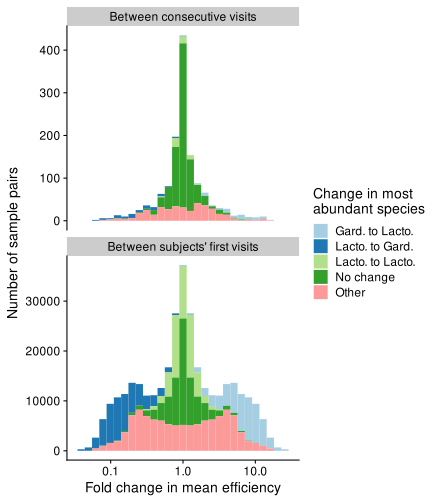
\includegraphics{figures/export-pdf/notebook/_posts/2021-11-01-momspi-summary/momspi-summary_files/figure-html5/momspi-mean-efficiency-fcs-1.pdf}
\caption{\label{fig:momspi-mean-efficiency-fcs}\textbf{Fold changes in the mean efficiency within and between women in the MOMS-PI study.}}
\end{figure}



\begin{figure}
\centering
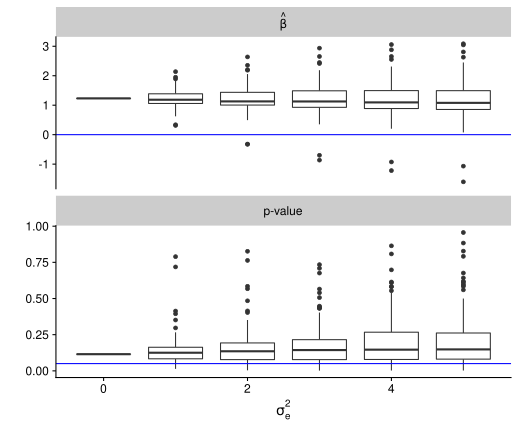
\includegraphics{figures/export-pdf/notebook/_posts/2021-10-18-evaluate-robustness-example/evaluate-robustness-example_files/figure-html5/summary_plot-1.pdf}
\caption{\label{fig:sensitivity-example}\textbf{A bias-sensivity analysis can be performed to examine how sensitive the results of a DA analysis are to assumptions about taxonomic bias in community measurements.} The figure shows the results of a bias-sensitivity analysis used to study the effect of bias on the association of \emph{Gardnerella vaginalis} and preterm birth that was investigated by Callahan et al. (\protect\hyperlink{ref-callahan2017repl}{2017}). 100 random efficiency vectors were drawn at 6 different bias strengths (quantified by the variance in log efficiency, \(\sigma_{e}^{2}\)). Each efficiency vector was used to calibrate the MGS profiles and perform a DA association test of \emph{G. vaginalis} versus the host's preterm birth outcome; regression coefficients \(\hat \beta\) indicate the increase of average logit proportion of \emph{G. vaginalis} in women who experienced preterm birth.}
\end{figure}



\hypertarget{references}{%
\section*{References}\label{references}}
\addcontentsline{toc}{section}{References}

\hypertarget{refs}{}
\begin{CSLReferences}{1}{0}
\leavevmode\vadjust pre{\hypertarget{ref-brooks2015thet}{}}%
Brooks, J Paul, David J Edwards, Michael D Harwich, Maria C Rivera, Jennifer M Fettweis, Myrna G Serrano, Robert A Reris, et al. 2015. {``{The truth about metagenomics: quantifying and counteracting bias in 16S rRNA studies}.''} \emph{BMC Microbiol.} BioMed Central. \url{https://doi.org/10.1186/s12866-015-0351-6}.

\leavevmode\vadjust pre{\hypertarget{ref-callahan2017repl}{}}%
Callahan, Benjamin J, Daniel B DiGiulio, Daniela S Aliaga Goltsman, Christine L Sun, Elizabeth K Costello, Pratheepa Jeganathan, Joseph R Biggio, et al. 2017. {``{Replication and refinement of a vaginal microbial signature of preterm birth in two racially distinct cohorts of US women}.''} \emph{Proc. Natl. Acad. Sci. U. S. A.} 114 (37): 9966--71. \url{https://doi.org/10.1073/pnas.1705899114}.

\leavevmode\vadjust pre{\hypertarget{ref-chng2020meta}{}}%
Chng, Kern Rei, Tarini Shankar Ghosh, Yi Han Tan, Tannistha Nandi, Ivor Russel Lee, Amanda Hui Qi Ng, Chenhao Li, et al. 2020. {``{Metagenome-wide association analysis identifies microbial determinants of post-antibiotic ecological recovery in the gut}.''} \emph{Nat. Ecol. Evol.} 4 (9): 1256--67. \url{https://doi.org/10.1038/s41559-020-1236-0}.

\leavevmode\vadjust pre{\hypertarget{ref-contijoch2019gutm}{}}%
Contijoch, Eduardo J, Graham J Britton, Chao Yang, Ilaria Mogno, Zhihua Li, Ruby Ng, Sean R Llewellyn, et al. 2019. {``{Gut microbiota density influences host physiology and is shaped by host and microbial factors}.''} \emph{Elife} 8 (January). \url{https://doi.org/10.7554/eLife.40553}.

\leavevmode\vadjust pre{\hypertarget{ref-cruz2021equi}{}}%
Cruz, Giuliano Netto Flores, Ana Paula Christoff, and Luiz Felipe Valter de Oliveira. 2021. {``{Equivolumetric Protocol Generates Library Sizes Proportional to Total Microbial Load in 16S Amplicon Sequencing}.''} \emph{Front. Microbiol.} 12 (February): 1--16. \url{https://doi.org/10.3389/fmicb.2021.638231}.

\leavevmode\vadjust pre{\hypertarget{ref-david2014host}{}}%
David, Lawrence A, Arne C Materna, Jonathan Friedman, Maria I Campos-Baptista, Matthew C Blackburn, Allison Perrotta, Susan E Erdman, and Eric J Alm. 2014. {``{Host lifestyle affects human microbiota on daily timescales}.''} \emph{Genome Biol.} 15 (7): R89. \url{https://doi.org/10.1186/gb-2014-15-7-r89}.

\leavevmode\vadjust pre{\hypertarget{ref-diener2021nonr}{}}%
Diener, Christian, Anna C. H. Hoge, Sean M. Kearney, Ulrike Kusebauch, Sushmita Patwardhan, Robert L. Moritz, Susan E. Erdman, and Sean M. Gibbons. 2021. {``{Non-responder phenotype reveals apparent microbiome-wide antibiotic tolerance in the murine gut}.''} \emph{Commun. Biol.} 4 (1). \url{https://doi.org/10.1038/s42003-021-01841-8}.

\leavevmode\vadjust pre{\hypertarget{ref-dreo2014opti}{}}%
Dreo, Tanja, Manca Pirc, Živa Ramšak, Jernej Pavšič, Mojca Milavec, Jana Žel, and Kristina Gruden. 2014. {``{Optimising droplet digital PCR analysis approaches for detection and quantification of bacteria: a case study of fire blight and potato brown rot}.''} \emph{Anal. Bioanal. Chem.} 406 (26): 6513--28. \url{https://doi.org/10.1007/s00216-014-8084-1}.

\leavevmode\vadjust pre{\hypertarget{ref-fettweis2019thev}{}}%
Fettweis, Jennifer M., Myrna G. Serrano, Jamie Paul Brooks, David J. Edwards, Philippe H. Girerd, Hardik I. Parikh, Bernice Huang, et al. 2019. {``{The vaginal microbiome and preterm birth}.''} \emph{Nat. Med.} 25 (6): 1012--21. \url{https://doi.org/10.1038/s41591-019-0450-2}.

\leavevmode\vadjust pre{\hypertarget{ref-finucane2014atax}{}}%
Finucane, Mariel M., Thomas J. Sharpton, Timothy J. Laurent, and Katherine S. Pollard. 2014. {``{A Taxonomic Signature of Obesity in the Microbiome? Getting to the Guts of the Matter}.''} Edited by Markus M. Heimesaat. \emph{PLoS One} 9 (1): e84689. \url{https://doi.org/10.1371/journal.pone.0084689}.

\leavevmode\vadjust pre{\hypertarget{ref-galazzo2020howt}{}}%
Galazzo, Gianluca, Niels van Best, Birke J. Benedikter, Kevin Janssen, Liene Bervoets, Christel Driessen, Melissa Oomen, et al. 2020. {``{How to Count Our Microbes? The Effect of Different Quantitative Microbiome Profiling Approaches}.''} \emph{Front. Cell. Infect. Microbiol.} 10 (August). \url{https://doi.org/10.3389/fcimb.2020.00403}.

\leavevmode\vadjust pre{\hypertarget{ref-gloor2017micr}{}}%
Gloor, Gregory B., Jean M. Macklaim, Vera Pawlowsky-Glahn, and Juan J. Egozcue. 2017. {``{Microbiome Datasets Are Compositional: And This Is Not Optional}.''} \emph{Front. Microbiol.} 8 (November): 2224. \url{https://doi.org/10.3389/fmicb.2017.02224}.

\leavevmode\vadjust pre{\hypertarget{ref-hardwick2018synt}{}}%
Hardwick, Simon A., Wendy Y. Chen, Ted Wong, Bindu S. Kanakamedala, Ira W. Deveson, Sarah E. Ongley, Nadia S. Santini, et al. 2018. {``{Synthetic microbe communities provide internal reference standards for metagenome sequencing and analysis}.''} \emph{Nat. Commun.} 9 (1): 3096. \url{https://doi.org/10.1038/s41467-018-05555-0}.

\leavevmode\vadjust pre{\hypertarget{ref-harrison2021theq}{}}%
Harrison, Joshua G., W. John Calder, Bryan Shuman, and C. Alex Buerkle. 2021. {``{The quest for absolute abundance: The use of internal standards for DNA‐based community ecology}.''} \emph{Mol. Ecol. Resour.} 21 (1): 30--43. \url{https://doi.org/10.1111/1755-0998.13247}.

\leavevmode\vadjust pre{\hypertarget{ref-ji2019quan}{}}%
Ji, Brian W., Ravi U. Sheth, Purushottam D. Dixit, Yiming Huang, Andrew Kaufman, Harris H. Wang, and Dennis Vitkup. 2019. {``{Quantifying spatiotemporal variability and noise in absolute microbiota abundances using replicate sampling}.''} \emph{Nat. Methods} 16 (8): 731--36. \url{https://doi.org/10.1038/s41592-019-0467-y}.

\leavevmode\vadjust pre{\hypertarget{ref-jian2020quan}{}}%
Jian, Ching, Panu Luukkonen, Hannele Yki-Järvinen, Anne Salonen, and Katri Korpela. 2020. {``{Quantitative PCR provides a simple and accessible method for quantitative microbiota profiling}.''} Edited by Ivone Vaz-Moreira. \emph{PLoS One} 15 (1): e0227285. \url{https://doi.org/10.1371/journal.pone.0227285}.

\leavevmode\vadjust pre{\hypertarget{ref-karasov2020ther}{}}%
Karasov, Talia L., Manuela Neumann, Alejandra Duque-Jaramillo, Sonja Kersten, Ilja Bezrukov, Birgit Schröppel, Efthymia Symeonidi, et al. 2020. {``{The relationship between microbial population size and disease in the Arabidopsis thaliana phyllosphere}.''} \emph{bioRxiv}. \url{https://doi.org/10.1101/828814}.

\leavevmode\vadjust pre{\hypertarget{ref-kevorkian2018esti}{}}%
Kevorkian, Richard, Jordan T Bird, Alexander Shumaker, and Karen G Lloyd. 2018. {``{Estimating Population Turnover Rates by Relative Quantification Methods Reveals Microbial Dynamics in Marine Sediment}.''} \emph{Appl. Environ. Microbiol.} 84 (1): e01443--17. \url{https://doi.org/10.1128/AEM.01443-17}.

\leavevmode\vadjust pre{\hypertarget{ref-korpela2018inte}{}}%
Korpela, Katri, Elin W. Blakstad, Sissel J. Moltu, Kenneth Strømmen, Britt Nakstad, Arild E. Rønnestad, Kristin Brække, Per O. Iversen, Christian A. Drevon, and Willem de Vos. 2018. {``{Intestinal microbiota development and gestational age in preterm neonates}.''} \emph{Sci. Rep.} 8 (1): 1--9. \url{https://doi.org/10.1038/s41598-018-20827-x}.

\leavevmode\vadjust pre{\hypertarget{ref-kumar2018anal}{}}%
Kumar, M. Senthil, Eric V. Slud, Kwame Okrah, Stephanie C. Hicks, Sridhar Hannenhalli, and Héctor Corrada Bravo. 2018. {``{Analysis and correction of compositional bias in sparse sequencing count data}.''} \emph{BMC Genomics} 19 (1): 799. \url{https://doi.org/10.1186/s12864-018-5160-5}.

\leavevmode\vadjust pre{\hypertarget{ref-leopold2020host}{}}%
Leopold, Devin R, and Posy E Busby. 2020. {``{Host Genotype and Colonist Arrival Order Jointly Govern Plant Microbiome Composition and Function}.''} \emph{Curr. Biol.} 30 (16): 3260--3266.e5. \url{https://doi.org/10.1016/j.cub.2020.06.011}.

\leavevmode\vadjust pre{\hypertarget{ref-lloyd2020evid}{}}%
Lloyd, Karen G., Jordan T. Bird, Joy Buongiorno, Emily Deas, Richard Kevorkian, Talor Noordhoek, Jacob Rosalsky, and Taylor Roy. 2020. {``{Evidence for a Growth Zone for Deep-Subsurface Microbial Clades in Near-Surface Anoxic Sediments}.''} \emph{Appl. Environ. Microbiol.} 86 (19): 1--15. \url{https://doi.org/10.1128/AEM.00877-20}.

\leavevmode\vadjust pre{\hypertarget{ref-lozupone2013meta}{}}%
Lozupone, Catherine A, Jesse Stombaugh, Antonio Gonzalez, Gail Ackermann, Janet K Jansson, Jeffrey I Gordon, Doug Wendel, Yoshiki Va, and Rob Knight. 2013. {``{Meta-analyses of studies of the human microbiota}.''} \emph{Genome Res.}, 1704--14. \url{https://doi.org/10.1101/gr.151803.112}.

\leavevmode\vadjust pre{\hypertarget{ref-mandal2015anal}{}}%
Mandal, Siddhartha, Will Van Treuren, Richard A. White, Merete Eggesbø, Rob Knight, and Shyamal D. Peddada. 2015. {``{Analysis of composition of microbiomes: a novel method for studying microbial composition}.''} \emph{Microb. Ecol. Heal. Dis.} 26 (1): 27663. \url{https://doi.org/10.3402/mehd.v26.27663}.

\leavevmode\vadjust pre{\hypertarget{ref-martin2020mode}{}}%
Martin, Bryan D., Daniela Witten, and Amy D. Willis. 2020. {``{Modeling microbial abundances and dysbiosis with beta-binomial regression}.''} \emph{Ann. Appl. Stat.} 14 (1): 94--115. \url{https://doi.org/10.1214/19-AOAS1283}.

\leavevmode\vadjust pre{\hypertarget{ref-mclaren2019cons}{}}%
McLaren, Michael R, Amy D Willis, and Benjamin J Callahan. 2019. {``{Consistent and correctable bias in metagenomic sequencing experiments}.''} \emph{Elife} 8 (September): 46923. \url{https://doi.org/10.7554/eLife.46923}.

\leavevmode\vadjust pre{\hypertarget{ref-morella2018rapi}{}}%
Morella, Norma M., Shangyang Christopher Yang, Catherine A. Hernandez, and Britt Koskella. 2018. {``{Rapid quantification of bacteriophages and their bacterial hosts in vitro and in vivo using droplet digital PCR}.''} \emph{J. Virol. Methods} 259 (May): 18--24. \url{https://doi.org/10.1016/j.jviromet.2018.05.007}.

\leavevmode\vadjust pre{\hypertarget{ref-pavsic2016digi}{}}%
Pavšič, Jernej, Jana Žel, and Mojca Milavec. 2016. {``{Digital PCR for direct quantification of viruses without DNA extraction}.''} \emph{Anal. Bioanal. Chem.} 408 (1): 67--75. \url{https://doi.org/10.1007/s00216-015-9109-0}.

\leavevmode\vadjust pre{\hypertarget{ref-props2017abso}{}}%
Props, Ruben, Frederiek-Maarten Kerckhof, Peter Rubbens, Jo De Vrieze, Emma Hernandez Sanabria, Willem Waegeman, Pieter Monsieurs, Frederik Hammes, and Nico Boon. 2017. {``{Absolute quantification of microbial taxon abundances}.''} \emph{ISME J.} 11 (2): 584--87. \url{https://doi.org/10.1038/ismej.2016.117}.

\leavevmode\vadjust pre{\hypertarget{ref-rao2021mult}{}}%
Rao, Chitong, Katharine Z. Coyte, Wayne Bainter, Raif S. Geha, Camilia R. Martin, and Seth Rakoff-Nahoum. 2021. {``{Multi-kingdom ecological drivers of microbiota assembly in preterm infants}.''} \emph{Nature} 591 (7851): 633--38. \url{https://doi.org/10.1038/s41586-021-03241-8}.

\leavevmode\vadjust pre{\hypertarget{ref-regalado2019comb}{}}%
Regalado, Julian, Derek S. Lundberg, Oliver Deusch, Sonja Kersten, Talia Karasov, Karin Poersch, Gautam Shirsekar, and Detlef Weigel. 2020. {``{Combining whole-genome shotgun sequencing and rRNA gene amplicon analyses to improve detection of microbe--microbe interaction networks in plant leaves}.''} \emph{ISME J.}, May, 823492. \url{https://doi.org/10.1038/s41396-020-0665-8}.

\leavevmode\vadjust pre{\hypertarget{ref-smets2016amet}{}}%
Smets, Wenke, Jonathan W. Leff, Mark A. Bradford, Rebecca L. McCulley, Sarah Lebeer, and Noah Fierer. 2016. {``{A method for simultaneous measurement of soil bacterial abundances and community composition via 16S rRNA gene sequencing}.''} \emph{Soil Biol. Biochem.} 96: 145--51. \url{https://doi.org/10.1016/j.soilbio.2016.02.003}.

\leavevmode\vadjust pre{\hypertarget{ref-stammler2016adju}{}}%
Stämmler, Frank, Joachim Gläsner, Andreas Hiergeist, Ernst Holler, Daniela Weber, Peter J. Oefner, André Gessner, and Rainer Spang. 2016. {``{Adjusting microbiome profiles for differences in microbial load by spike-in bacteria}.''} \emph{Microbiome} 4 (1): 28. \url{https://doi.org/10.1186/s40168-016-0175-0}.

\leavevmode\vadjust pre{\hypertarget{ref-tettamantiboshier2020comp}{}}%
Tettamanti Boshier, Florencia A., Sujatha Srinivasan, Anthony Lopez, Noah G. Hoffman, Sean Proll, David N. Fredricks, and Joshua T. Schiffer. 2020. {``{Complementing 16S rRNA Gene Amplicon Sequencing with Total Bacterial Load To Infer Absolute Species Concentrations in the Vaginal Microbiome}.''} \emph{mSystems} 5 (2): 1--14. \url{https://doi.org/10.1128/mSystems.00777-19}.

\leavevmode\vadjust pre{\hypertarget{ref-tkacz2018abso}{}}%
Tkacz, Andrzej, Marion Hortala, and Philip S. Poole. 2018. {``{Absolute quantitation of microbiota abundance in environmental samples}.''} \emph{Microbiome} 6 (1): 110. \url{https://doi.org/10.1186/s40168-018-0491-7}.

\leavevmode\vadjust pre{\hypertarget{ref-vandeputte2017quan}{}}%
Vandeputte, Doris, Gunter Kathagen, Kevin D'hoe, Sara Vieira-Silva, Mireia Valles-Colomer, João Sabino, Jun Wang, et al. 2017. {``{Quantitative microbiome profiling links gut community variation to microbial load}.''} \emph{Nature} 551 (7681): 507. \url{https://doi.org/10.1038/nature24460}.

\leavevmode\vadjust pre{\hypertarget{ref-vaninsberghe2020diar}{}}%
VanInsberghe, David, Joseph A. Elsherbini, Bernard Varian, Theofilos Poutahidis, Susan Erdman, and Martin F. Polz. 2020. {``{Diarrhoeal events can trigger long-term Clostridium difficile colonization with recurrent blooms}.''} \emph{Nat. Microbiol.} 5 (4): 642--50. \url{https://doi.org/10.1038/s41564-020-0668-2}.

\leavevmode\vadjust pre{\hypertarget{ref-wallace2021thed}{}}%
Wallace, Megan A., Kelsey A. Coffman, Clément Gilbert, Sanjana Ravindran, Gregory F. Albery, Jessica Abbott, Eliza Argyridou, et al. 2021. {``{The discovery, distribution, and diversity of DNA viruses associated with Drosophila melanogaster in Europe}.''} \emph{Virus Evol.} 7 (1): 1--23. \url{https://doi.org/10.1093/ve/veab031}.

\leavevmode\vadjust pre{\hypertarget{ref-wang2021curr}{}}%
Wang, Xiaofan, Samantha Howe, Feilong Deng, and Jiangchao Zhao. 2021. {``{Current Applications of Absolute Bacterial Quantification in Microbiome Studies and Decision-Making Regarding Different Biological Questions}.''} \emph{Microorganisms} 9 (9): 1797. \url{https://doi.org/10.3390/microorganisms9091797}.

\leavevmode\vadjust pre{\hypertarget{ref-wasserman2004allo}{}}%
Wasserman, Larry. 2004. \emph{{All of Statistics}}. Springer Texts in Statistics. New York, NY: Springer New York. \url{https://doi.org/10.1007/978-0-387-21736-9}.

\leavevmode\vadjust pre{\hypertarget{ref-yeh2018taxo}{}}%
Yeh, Yi-Chun, David M. Needham, Ella T. Sieradzki, and Jed A. Fuhrman. 2018. {``{Taxon Disappearance from Microbiome Analysis Reinforces the Value of Mock Communities as a Standard in Every Sequencing Run}.''} \emph{mSystems} 3 (3): e00023--18. \url{https://doi.org/10.1128/mSystems.00023-18}.

\leavevmode\vadjust pre{\hypertarget{ref-zemb2020abso}{}}%
Zemb, Olivier, Caroline S Achard, Jerome Hamelin, Marie‐Léa De Almeida, Béatrice Gabinaud, Laurent Cauquil, Lisanne M. G. Verschuren, and Jean-jacques Godon. 2020. {``{Absolute quantitation of microbes using 16S rRNA gene metabarcoding: A rapid normalization of relative abundances by quantitative PCR targeting a 16S rRNA gene spike‐in standard}.''} \emph{Microbiologyopen} 9 (3): 1--21. \url{https://doi.org/10.1002/mbo3.977}.

\end{CSLReferences}

\end{document}
